\documentclass[12pt]{book}
\usepackage[utf8]{inputenc}
\usepackage[T1]{fontenc}
\usepackage{lmodern}
\usepackage{xcolor}
\usepackage{listings}
\usepackage{amsmath}
\usepackage[hidelinks]{hyperref}
\usepackage[skip=10pt plus1pt, indent=20pt]{parskip}
\usepackage[spanish]{babel}
\usepackage[a4paper, margin=2.5cm]{geometry}
\usepackage{graphicx}
\usepackage{comment}

\newcommand{\questionb}[1]{\bigskip {\large \item \emph{#1}}\bigskip}

\renewcommand\lstlistingname{Código}
\renewcommand\lstlistlistingname{Códigos}

\lstdefinelanguage{Rust}{%
  sensitive%
, morecomment=[l]{//}%
, morecomment=[s]{/*}{*/}%
, moredelim=[s][{\itshape\color[rgb]{0,0,0.75}}]{\#[}{]}%
, morestring=[b]{"}%
, alsodigit={}%
, alsoother={}%
, alsoletter={!}%
, morekeywords={break, continue, else, for, if, in, loop, match, return, while}  % control flow keywords
, morekeywords={as, const, let, move, mut, ref, static}  % in the context of variables
, morekeywords={dyn, enum, fn, impl, Self, self, struct, trait, type, union, use, where}  % in the context of declarations
, morekeywords={crate, extern, mod, pub, super}  % in the context of modularisation
, morekeywords={unsafe}  % markers
, morekeywords={abstract, alignof, become, box, do, final, macro, offsetof, override, priv, proc, pure, sizeof, typeof, unsized, virtual, yield}  % reserved identifiers
}%

\lstdefinestyle{colouredRust}%
{ keywordstyle=[2]\color[rgb]{0.75, 0, 0}% traits
, keywordstyle=[3]\color[rgb]{0, 0.5, 0}% primitive types
, keywordstyle=[4]\color[rgb]{0, 0.5, 0}% type and value constructors
, keywordstyle=[5]\color[rgb]{0, 0, 0.75}% macros
}%

\lstdefinestyle{boxed}{
  numbers=left%
, firstnumber=auto%
, numberblanklines=true%
, frame=trbL%
, numberstyle=\tiny%
, frame=leftline%
, numbersep=7pt%
, framesep=5pt%
, framerule=10pt%
, xleftmargin=15pt%
, backgroundcolor=\color[gray]{0.97}%
, rulecolor=\color[gray]{0.90}%
}

\lstset{
    basicstyle=\ttfamily\small,
    columns=fullflexible,
    keepspaces=true,
    showstringspaces=false,
    commentstyle=\color[gray]{0.4},
    stringstyle=\color[rgb]{0, 0, 0.5},
    frame=single,
    breakatwhitespace=true,
    breaklines=true,
    tabsize=4
}

\title{
    {Cuaderno de laboratorio}\\
    {\normalsize Laboratorio de Desarrollo de Hardware}
}
\author{Alejandro Domínguez Muñoz}
\date{Enero 2023}

\begin{document}

\maketitle

\tableofcontents

\part{Plataformas de desarrollo}

\graphicspath{{./1/}}

\chapter{Arduino}

\section{Activar luz desde el puerto serie}

Para activar una luz desde una placa Arduino, usaremos un relé que active una
luz alimentada externamente. El montaje quedaría como se muestra en la
fotografía:

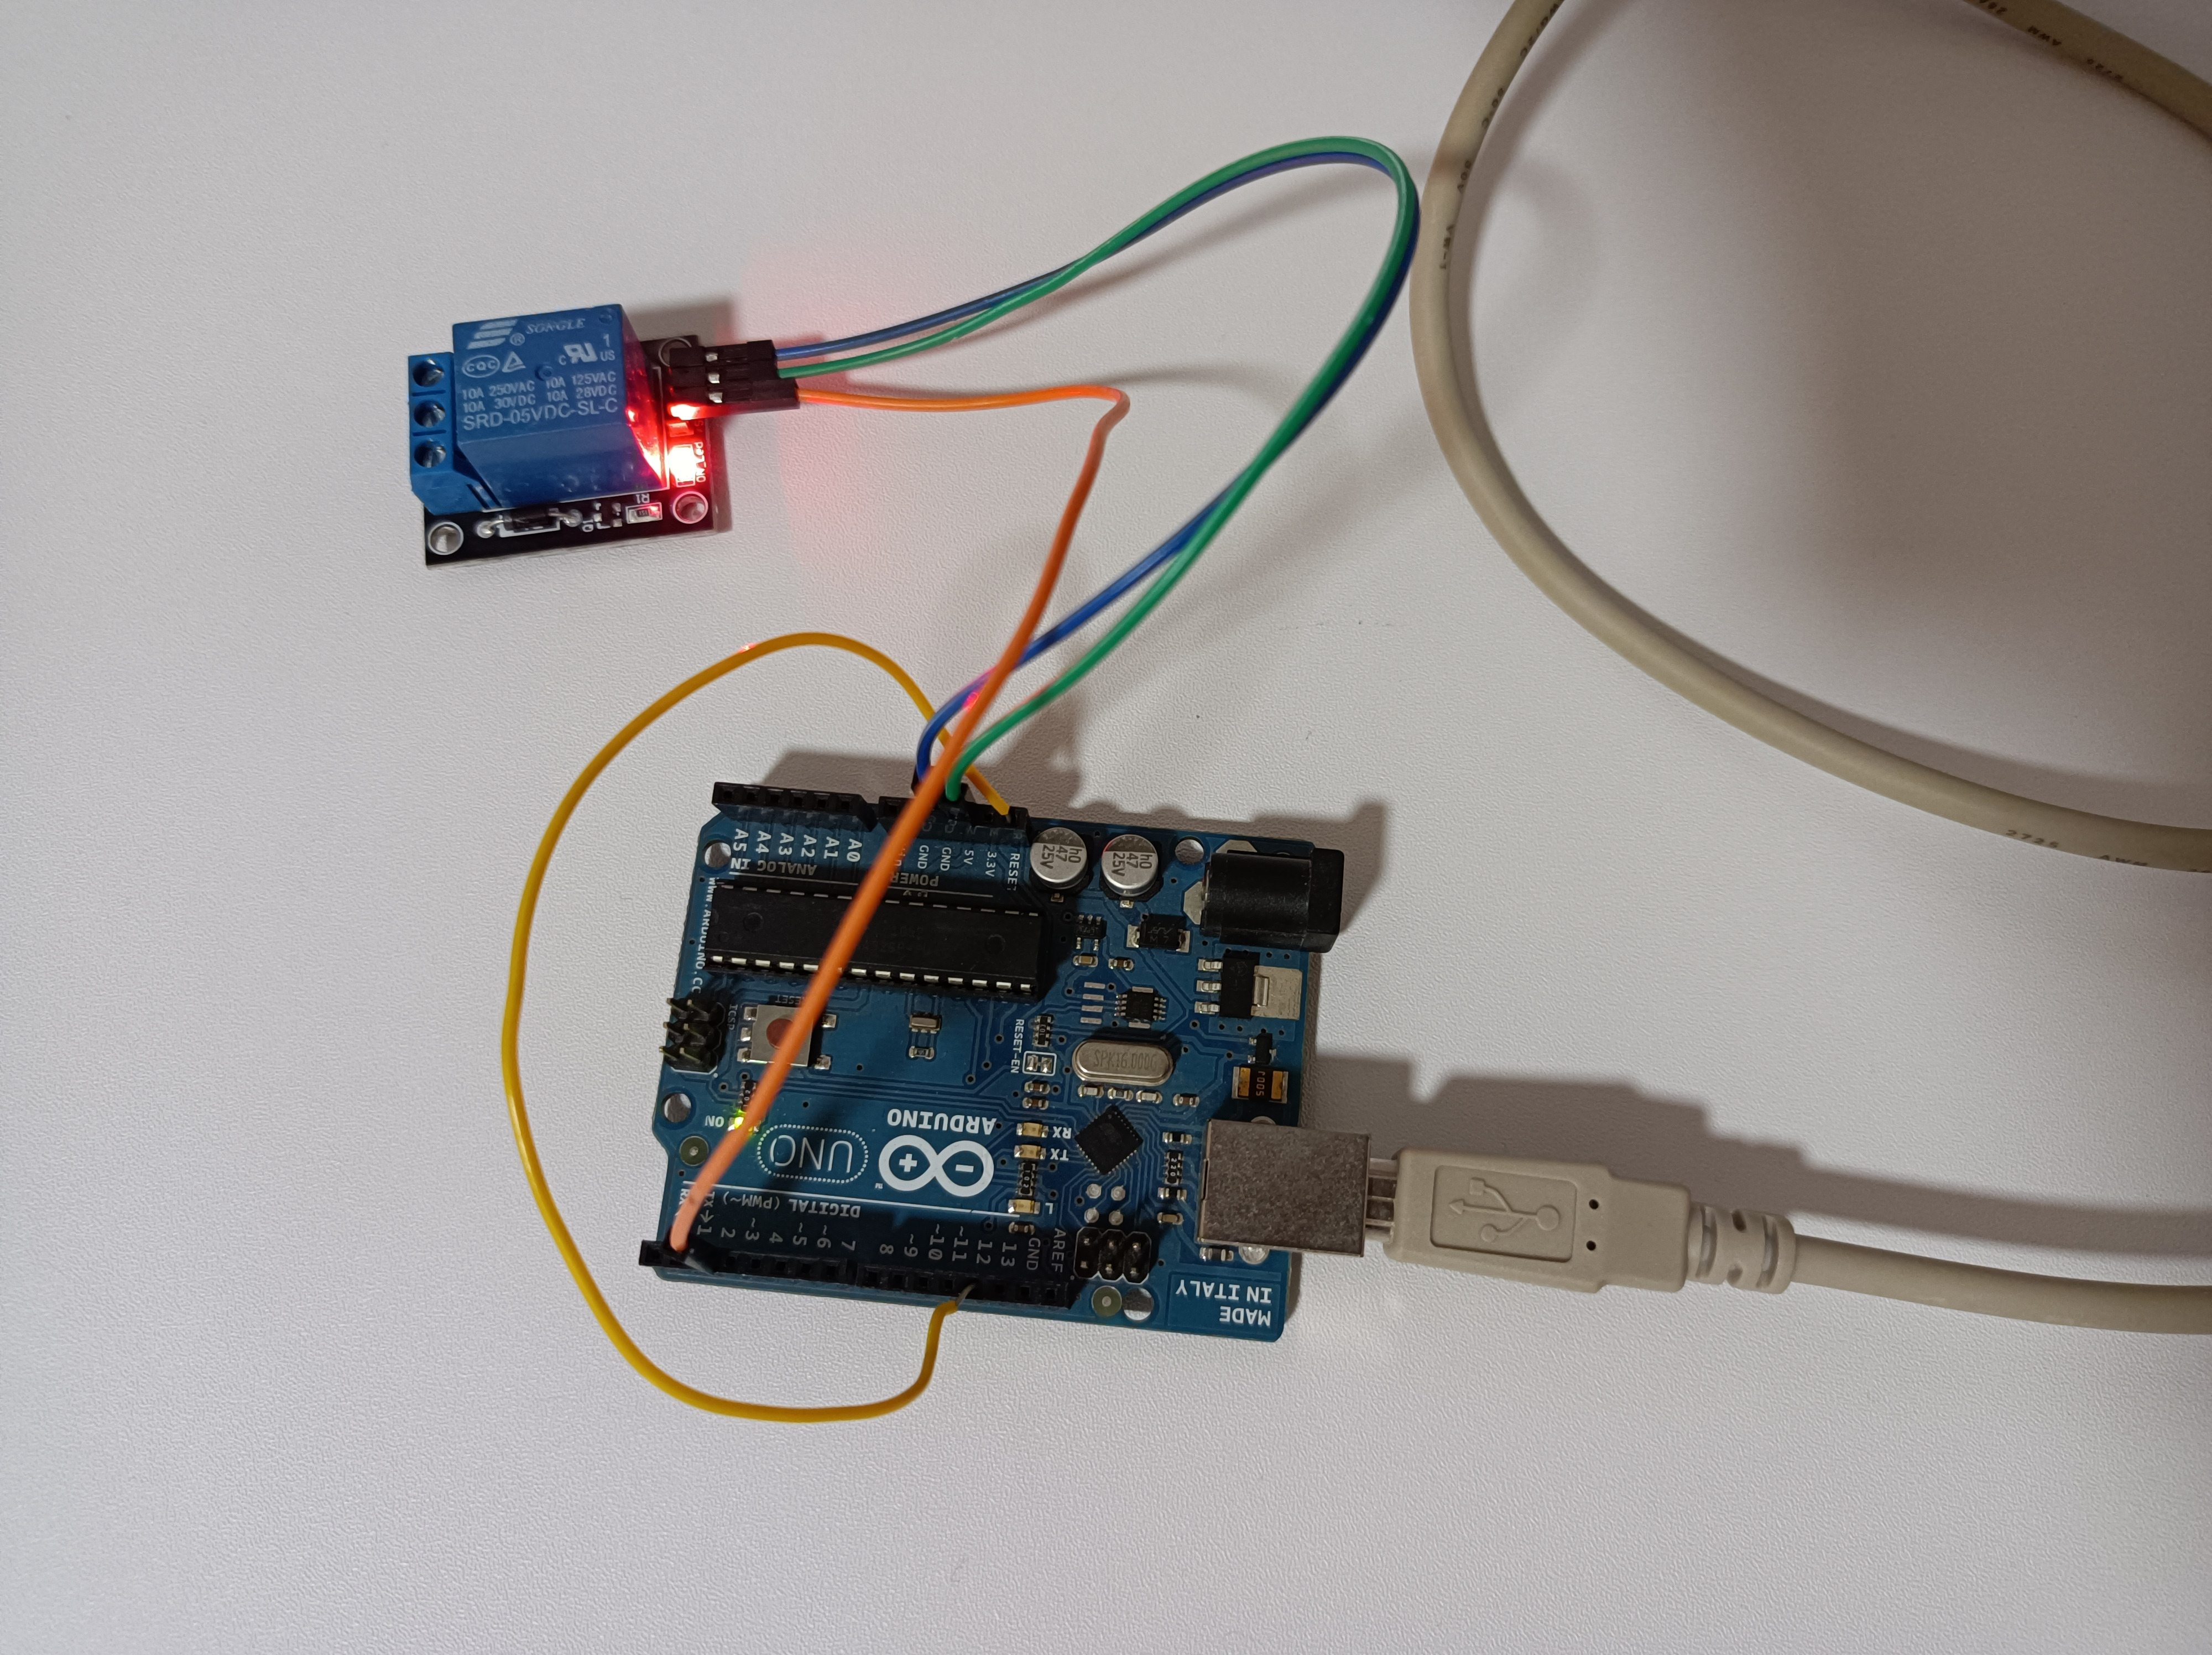
\includegraphics[width=\linewidth]{switch-light-wiring.jpg}

Programaremos la placa para que active los pines adecuados y procese las
señales que reciba por el puerto serie de manera que active el puerto serie a
9.600 bps y active el relé en caso de recibir el carácter \verb|h| y los
desactive en caso de recibir el carácter \verb|l|:

\lstinputlisting[language=C++, caption=switch-light.ino]{
    1/switch-light/switch-light.ino
}

Finalmente, desde el ordenador se enviará por el puerto serie solo las letras
\verb|h| y \verb|l| en caso de ser pulsadas, no otras, y si se pulsa \verb|q|
entonces se cerrará el programa cliente. Para ello, usaremos el lenguaje Rust
con el gestor de paquetes estándar Cargo. Estos componentes se instalan según
las indicaciones en su página
web\footnote{\url{https://www.rust-lang.org/es/tools/install}} en función del
sistema operativo que se esté usando, a través del gestor de instalaciones
Rustup. Se ha elegido este lenguaje dado que, aún estando orientado a la
programación de sistemas, garantiza que la gestión de la memoria es segura dado
que la comprueba en tiempo de compilación, esto a costa de no permitir ciertas
formas de realizar el control del flujo de ejecución.

La creación del proyecto del programa cliente se realiza ejecutando el comando
\lstinline{cargo new --vcs none nombre-del-proyecto}. En nuestro caso lo
llamaremos \verb|switch-light|, por lo que la instrucción a ejecutar será
\lstinline{cargo new --vcs none switch-light}. Esto creará una carpeta con el
nombre del mismo proyecto en el directorio desde el cual hayamos ejecutado la
instrucción, sin habilitar ningún sistema de control de versiones. Dentro de
dicha carpeta se formará una estructura de ficheros y directorios. Nos
interesan dos archivos. Por un lado está \verb|Cargo.toml|, que declara los
metadatos del proyecto y los paquetes de los que depende, con una versión
específica. Solo necesitamos añadir las dependencias después del marcador
\lstinline{[dependencies]}. Usaremos las librerías \verb|serialport|, para usar
los puertos serie del sistema, abstrayendo las diferencias entre sistemas
operativos, y \verb|console|, para acceder a características más avanzadas de
la terminal que las que proporciona la librería estándar. Este sería el
resultado:

\lstinputlisting[caption=switch-light/Cargo.toml]{
    1/switch-light/Cargo.toml
}

La versión de cada dependencia debe indicarse para evitar que cambios en la API
de las librerías impidan la compilación de la aplicación o que ésta se ejecute
de una forma inesperada.

El código del programa para realizar el comportamiento que se busca, descrito
anteriormente, es el siguiente:

\lstinputlisting[language=Rust, caption=switch-light/src/main.rs]{
    1/switch-light/src/main.rs
}

La constante \verb|PORT_PATH| debe ajustarse a la ruta del nodo de dispositivo
adecuado en Linux o al nombre del puerto donde esté conectada la placa Arduino
en el caso de Windows.

Sin embargo, hay que tener en cuenta que, como aparece comentado en el código
para la placa, en Linux hay que mantener el pin de Reset en alto, por lo que
hay que conectar dicho pin a otro que esté situado en alto, en nuestro caso el
pin 12, \emph{después de conectar la placa}, y en caso de que vaya a ser
reprogramada hay que dejar el pin de Reset libre. Esto ocurre porque Linux
envía una señal de control al abrir el puerto que Arduino interpreta como un
reset, incluso aunque se ajuste el puerto para que no envíe señales de
control\footnotemark. En Windows esto no pasa, por lo que no es necesario. El
setup mostrado ya tiene en cuenta esto, dado que se ha realizado sobre Linux.

\footnotetext{\url{https://unix.stackexchange.com/a/543527}}

Para ejecutar el programa (y compilarlo si es necesario), el comando a teclear
es \lstinline{cargo run}, dentro de la carpeta del proyecto.

En los siguientes ejercicios no se explicarán con tanto detalle las
instrucciones a ejecutar, dado que siempre siguen unos patrones muy similares.

\section{Control de servo desde el puerto serie}

Para controlar el giro de un servo de una placa Arduino, realizaremos las
siguientes conexiones:

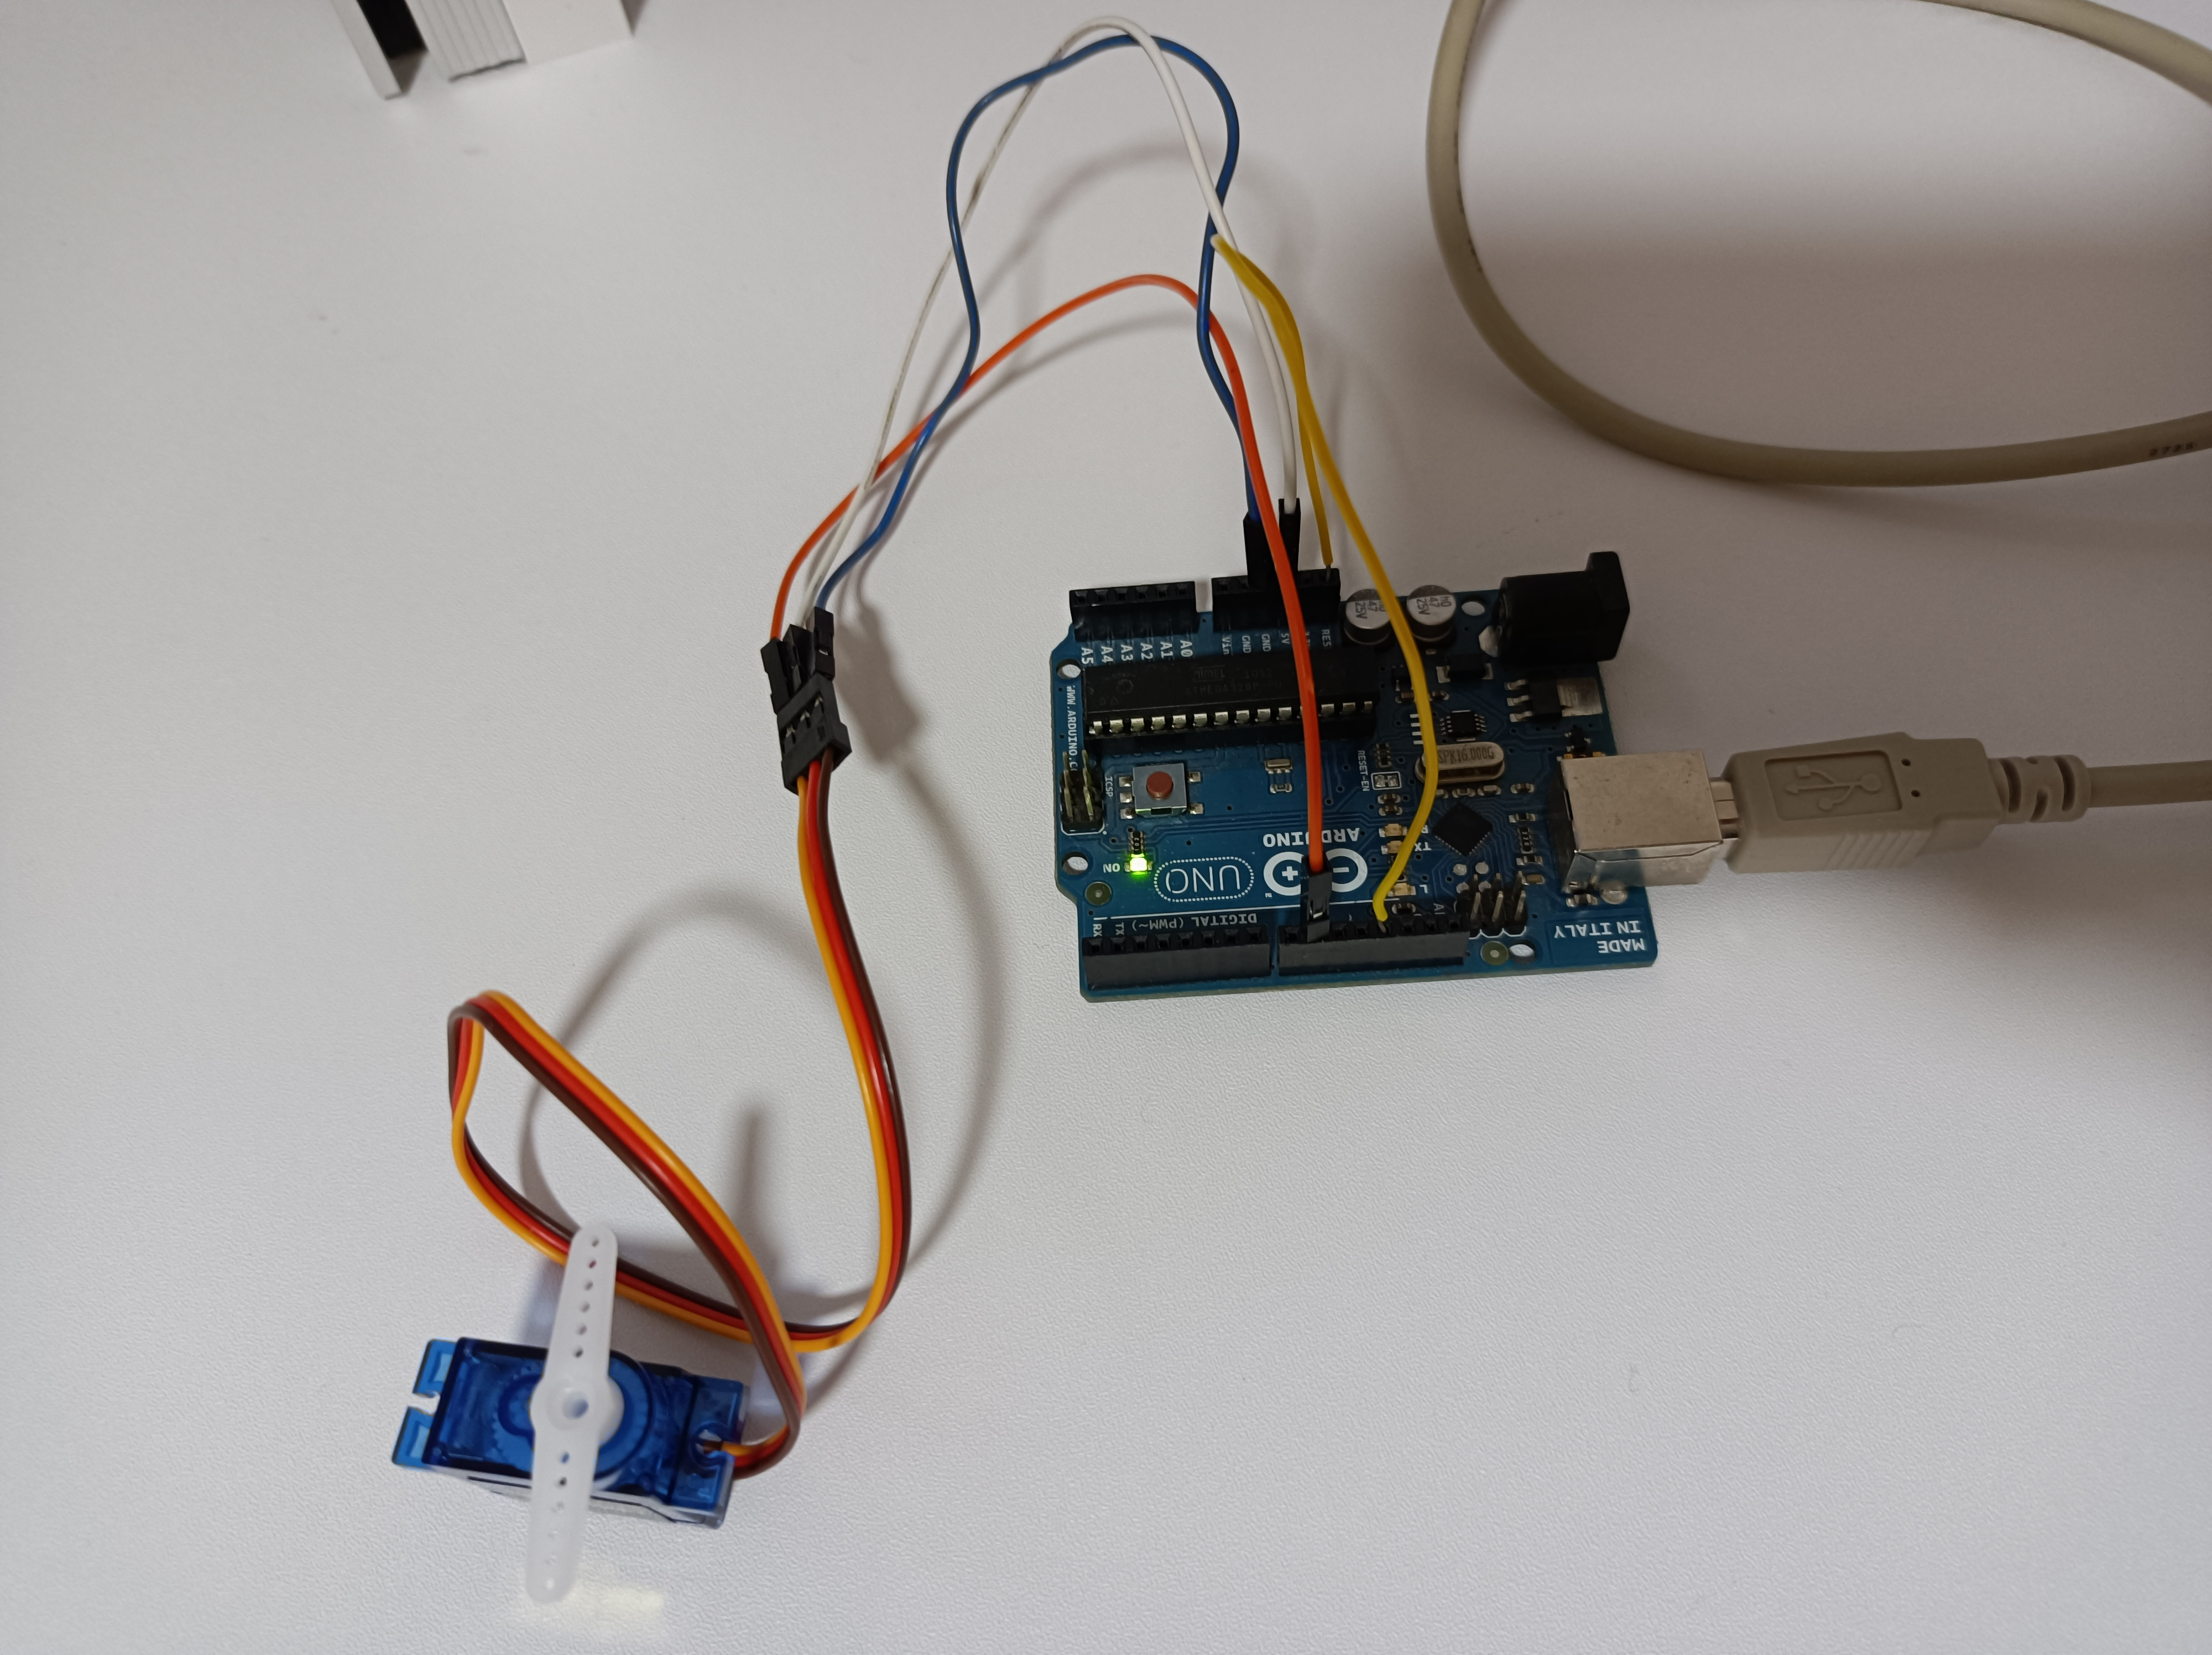
\includegraphics[width=\linewidth]{turn-servo-wiring.jpg}

La placa recibirá el valor en un byte bruto por el puerto serie y lo aplicará
directamente con ayuda de la librería que hace de controlador del motor.

\lstinputlisting[language=C++, caption=turn-servo.ino]{
    1/turn-servo/turn-servo.ino
}

Desde el ordenador se enviará por el puerto serie el valor en bruto,
validando la entrada para que no envíe valores que no estén entre 0 y 180.
Para este ejercicio no necesitamos la librería \verb|console|, por lo que
podemos prescindir de ella. Llamaremos al proyecto del programa cliente
\verb|turn-servo|.

\lstinputlisting[caption=turn-servo/Cargo.toml]{
    1/turn-servo/Cargo.toml
}

\lstinputlisting[language=Rust, caption=turn-servo/src/main.rs]{
    1/turn-servo/src/main.rs
}

\section{Mostrar datos del puerto serie en el display LCD}

En este ejercicio vamos a mostrar los caracteres que se envíen a través del
puerto serie por un display LCD controlado desde la placa de Arduino. Para ello
las conexiones se dispondrán de la manera que se muestra aquí:

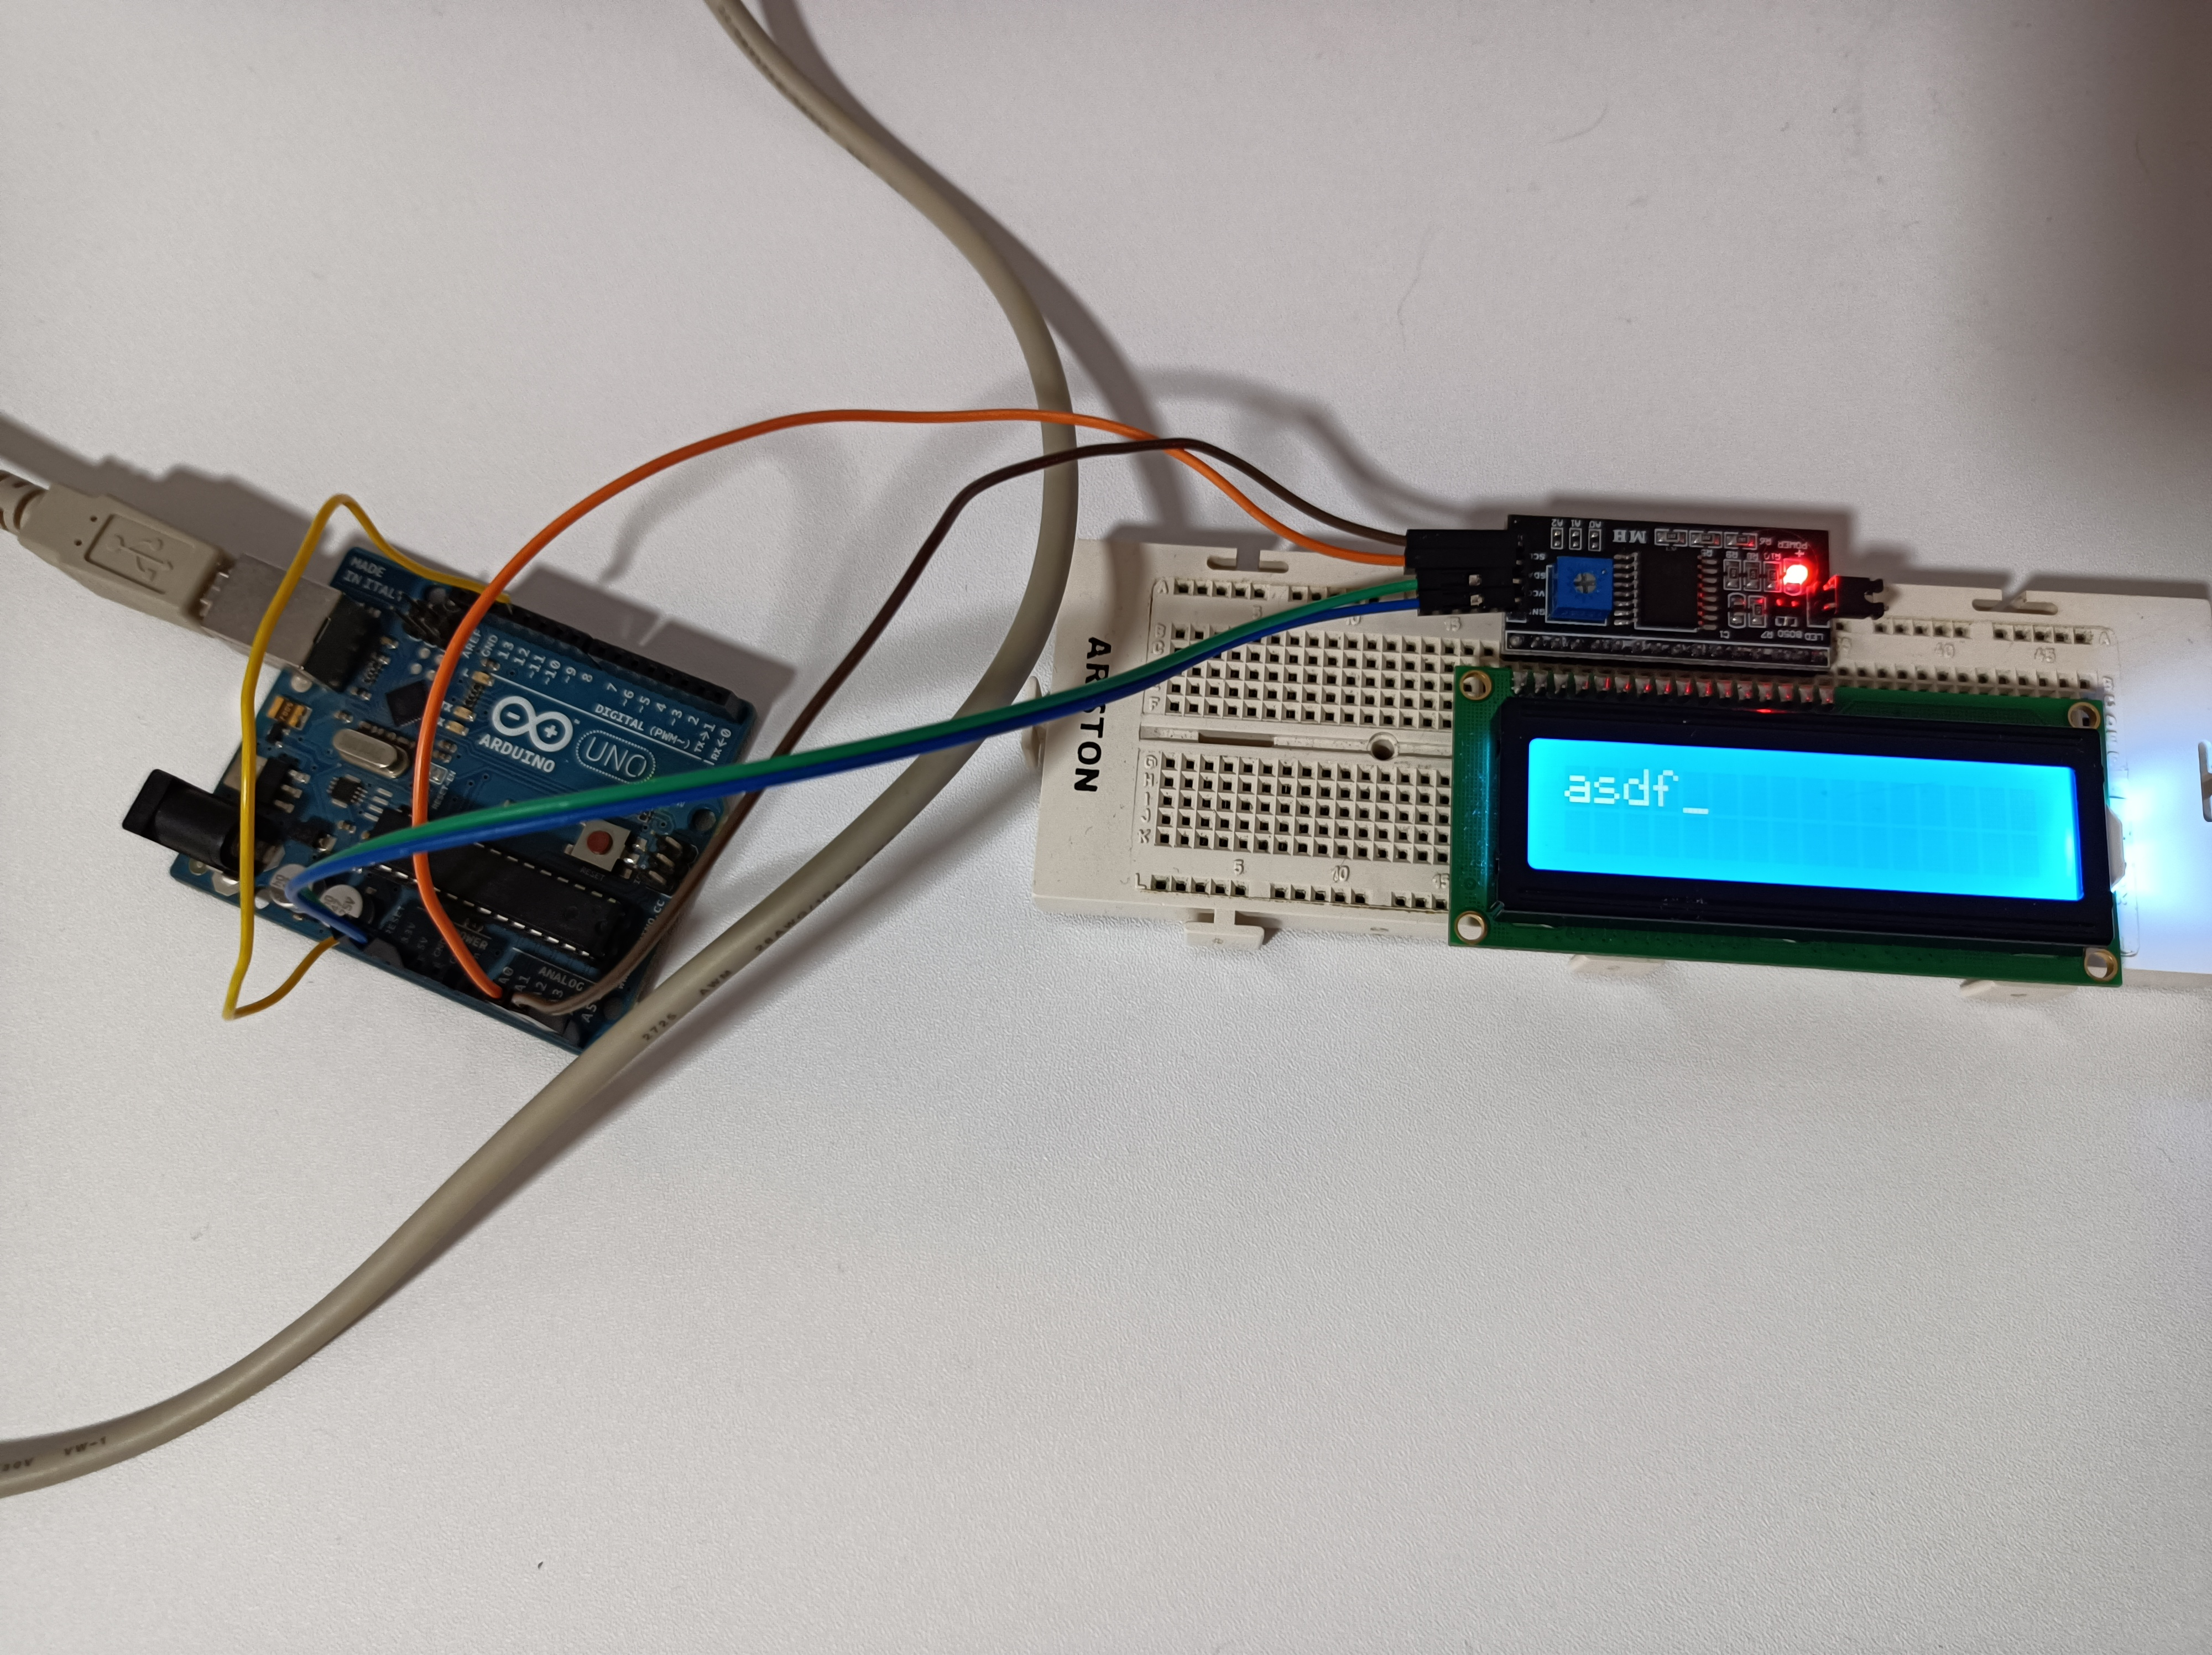
\includegraphics[width=\linewidth]{chars-display-wiring.jpg}

Usaremos la librería \verb|LiquidCrystal_I2C|\footnotemark que gestiona por
nosotros la comunicación con el display a través del bus I2C. Solo nos queda
reenviar los datos recibidos al driver del LCD:

\footnotetext{\url{
    https://github.com/johnrickman/LiquidCrystal_I2C/archive/refs/tags/1.1.3.zip
}}

\lstinputlisting[language=C++, caption=chars-display.ino]{
    1/chars-display/chars-display.ino
}

La aplicación cliente tiene una pequeña complicación, y es que no puede
cerrarse con la pulsación de una tecla. La forma más sencilla es aprovechar
el mecanismo de señal de cierre del sistema operativo, el cual emite dicho
mensaje a la aplicación al presionar la combinación de teclas \verb|Ctrl-C|.
Podemos acceder a esta funcionalidad con la librería \verb|ctrlc|. Llamaremos
al proyecto \verb|chars-display|.

\lstinputlisting[caption=chars-display/Cargo.toml]{
    1/chars-display/Cargo.toml
}

El código de la aplicación cliente se vuelve así muy sencillo:

\lstinputlisting[language=Rust, caption=chars-display/src/main.rs]{
    1/chars-display/src/main.rs
}

\section{Mostrar temperatura en el display LCD}

Aquí mostraremos la temperatura ambiente a la placa Arduino directamente en el
display LCD, sin comunicarse con otros dispositivos. El montaje es el que
sigue:

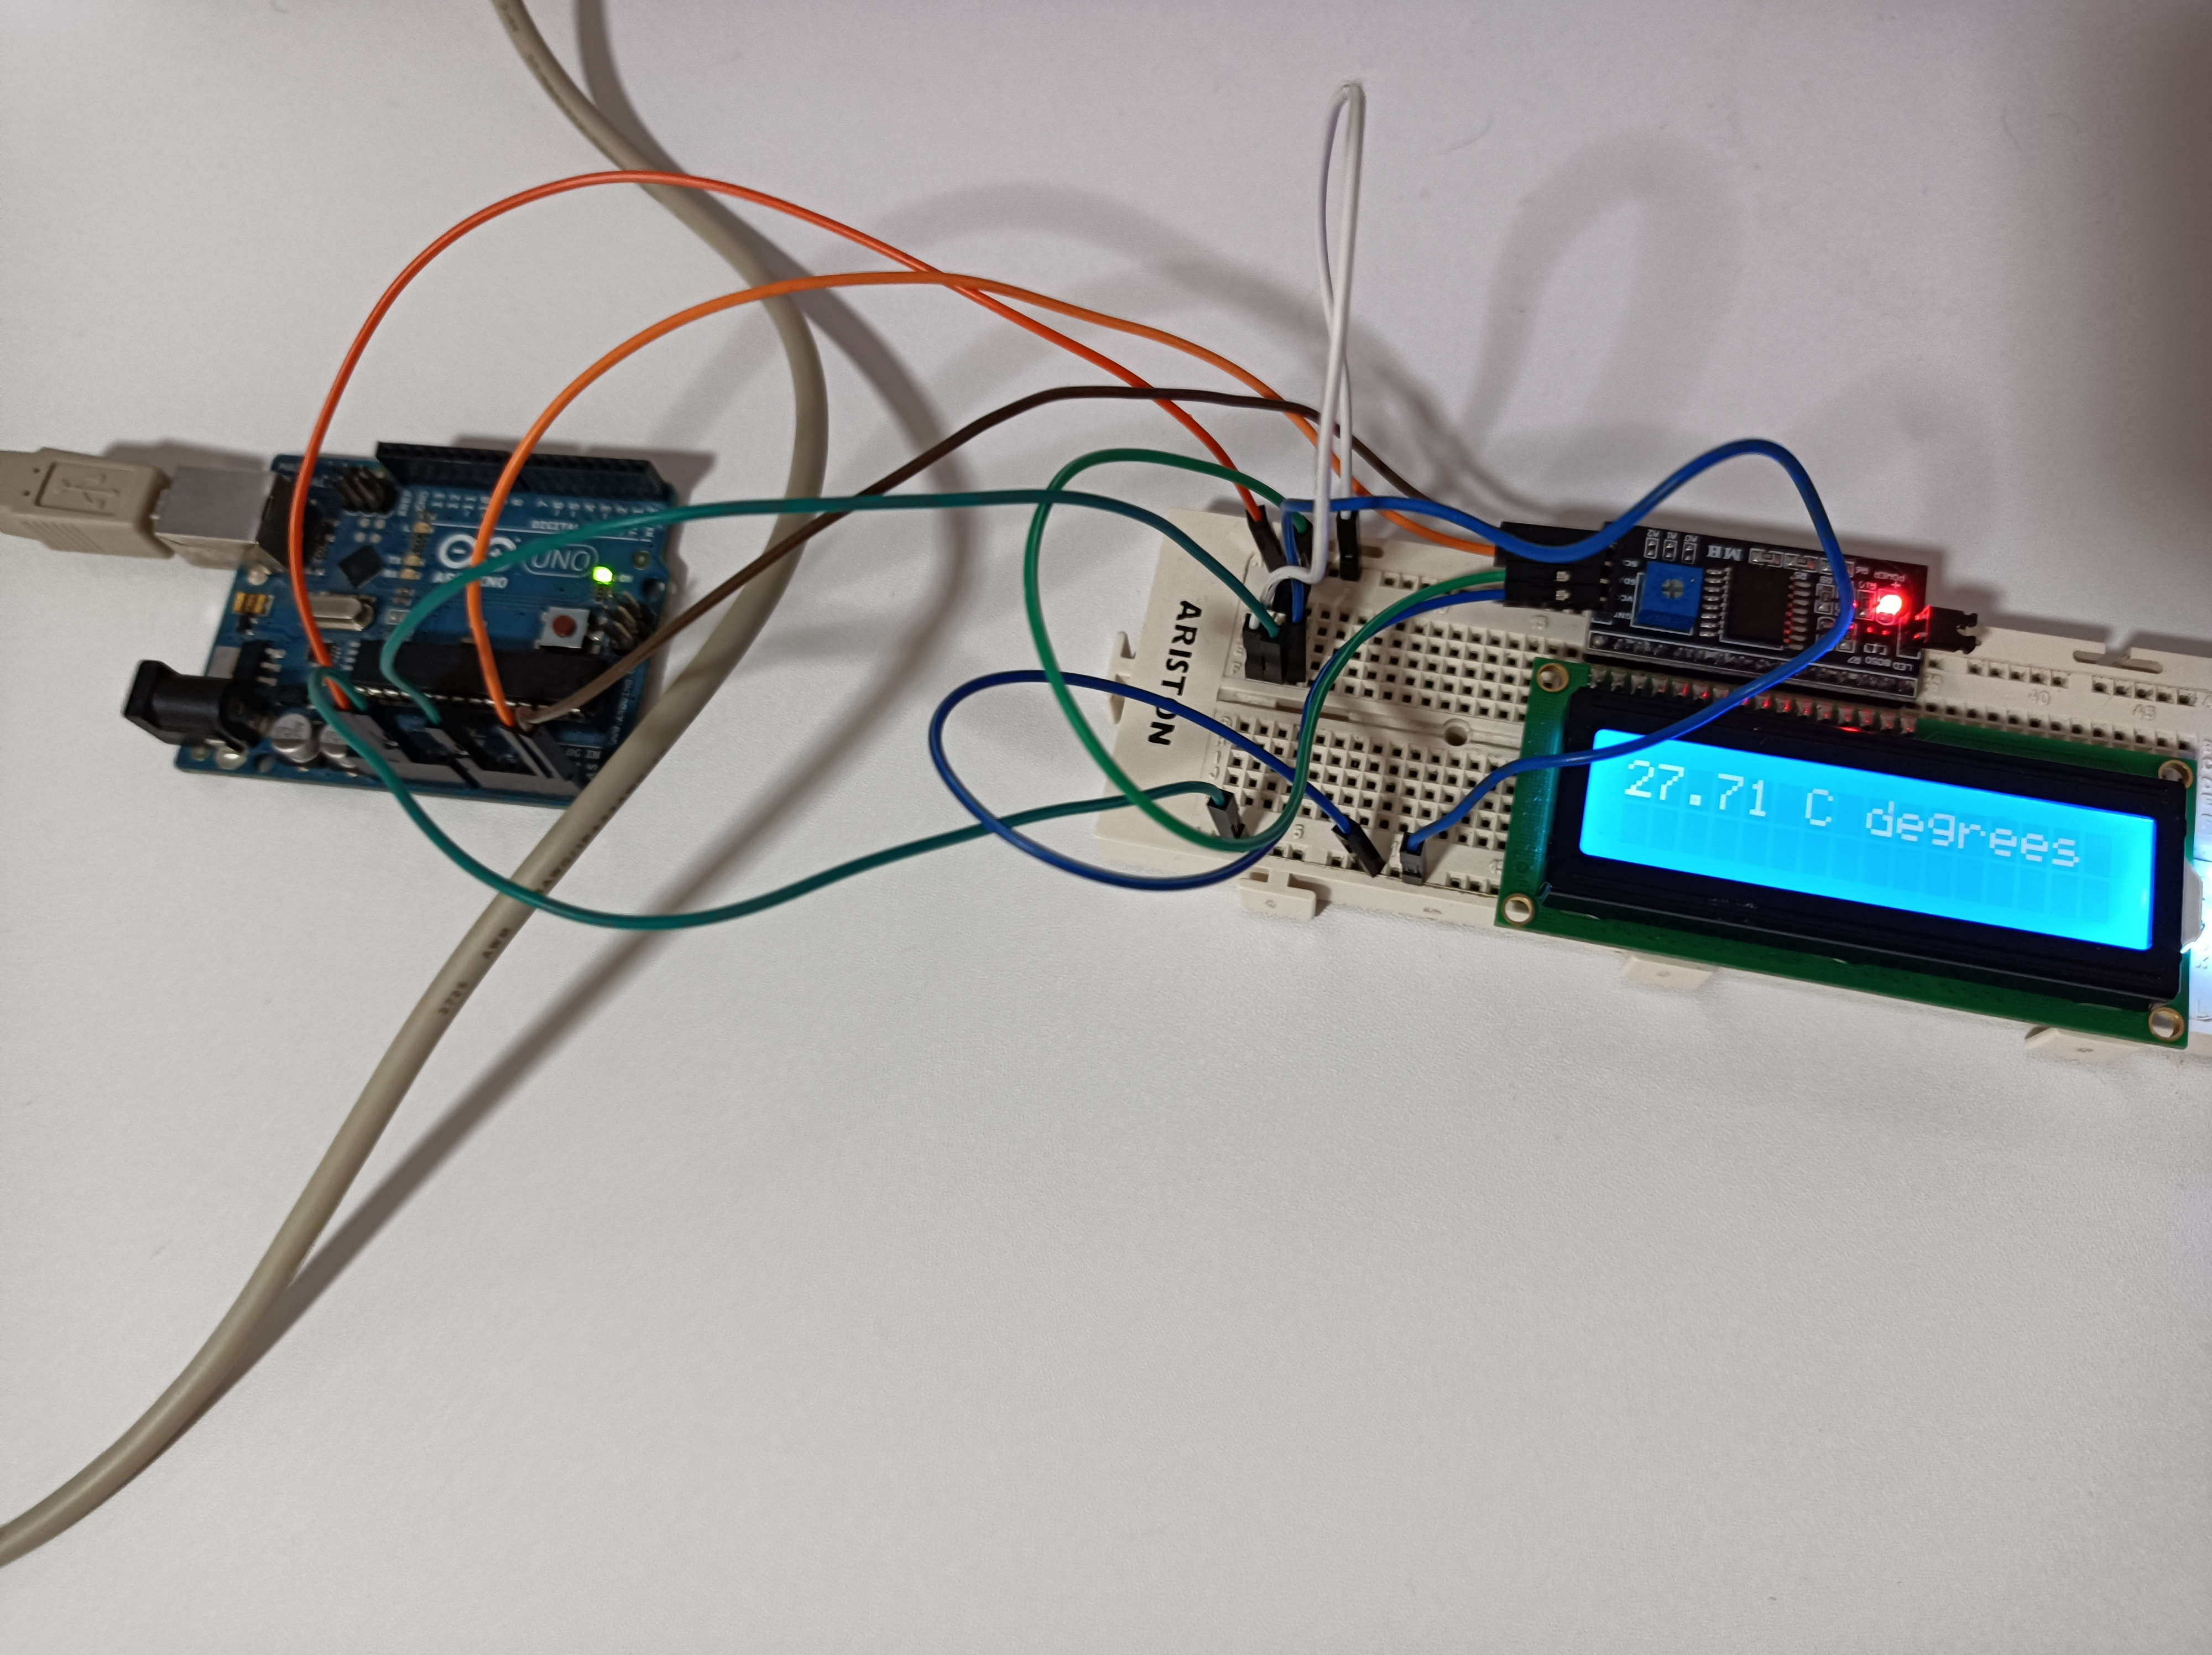
\includegraphics[width=\linewidth]{temperature-display-wiring.jpg}

Para traducir las mediciones de tensión en cifras de temperatura hay que
aplicar la siguiente fórmula:

\begin{equation*}
T = 100V - 50
\end{equation*}

Donde $V$ es la medición en \emph{voltios} y $T$ la cifra de temperatura.

Esto a su vez requiere traducir la medición numérica de la entrada analógica en
una cifra que refleje la magnitud en \emph{voltios}. Esta es la expresión que
define esta transformación:

\begin{equation*}
V = \frac{D}{D_{max}} \cdot V_{max}
\end{equation*}

Donde $D$ es la lectura conseguida, $V_{max}$ la tensión máxima que soporta el
pin analógico (que en este caso son \emph{5 V}) y $D_{max}$ la lectura máxima
que puede devolver el puerto (que en este caso es \emph{1023}).

Con esta información, así se programaría la placa Arduino para cumplir el
propósito establecido:

\lstinputlisting[language=C++, caption=temperature-display.ino]{
    1/temperature-display/temperature-display.ino
}

\section{Mostrar luz en el display LCD y en el puerto serie}

En este ejercicio mediremos la luz ambiente mostrándola por el display LCD y
enviándola por ordenador al mismo tiempo usando un fotorresistor. Este es el
montaje:

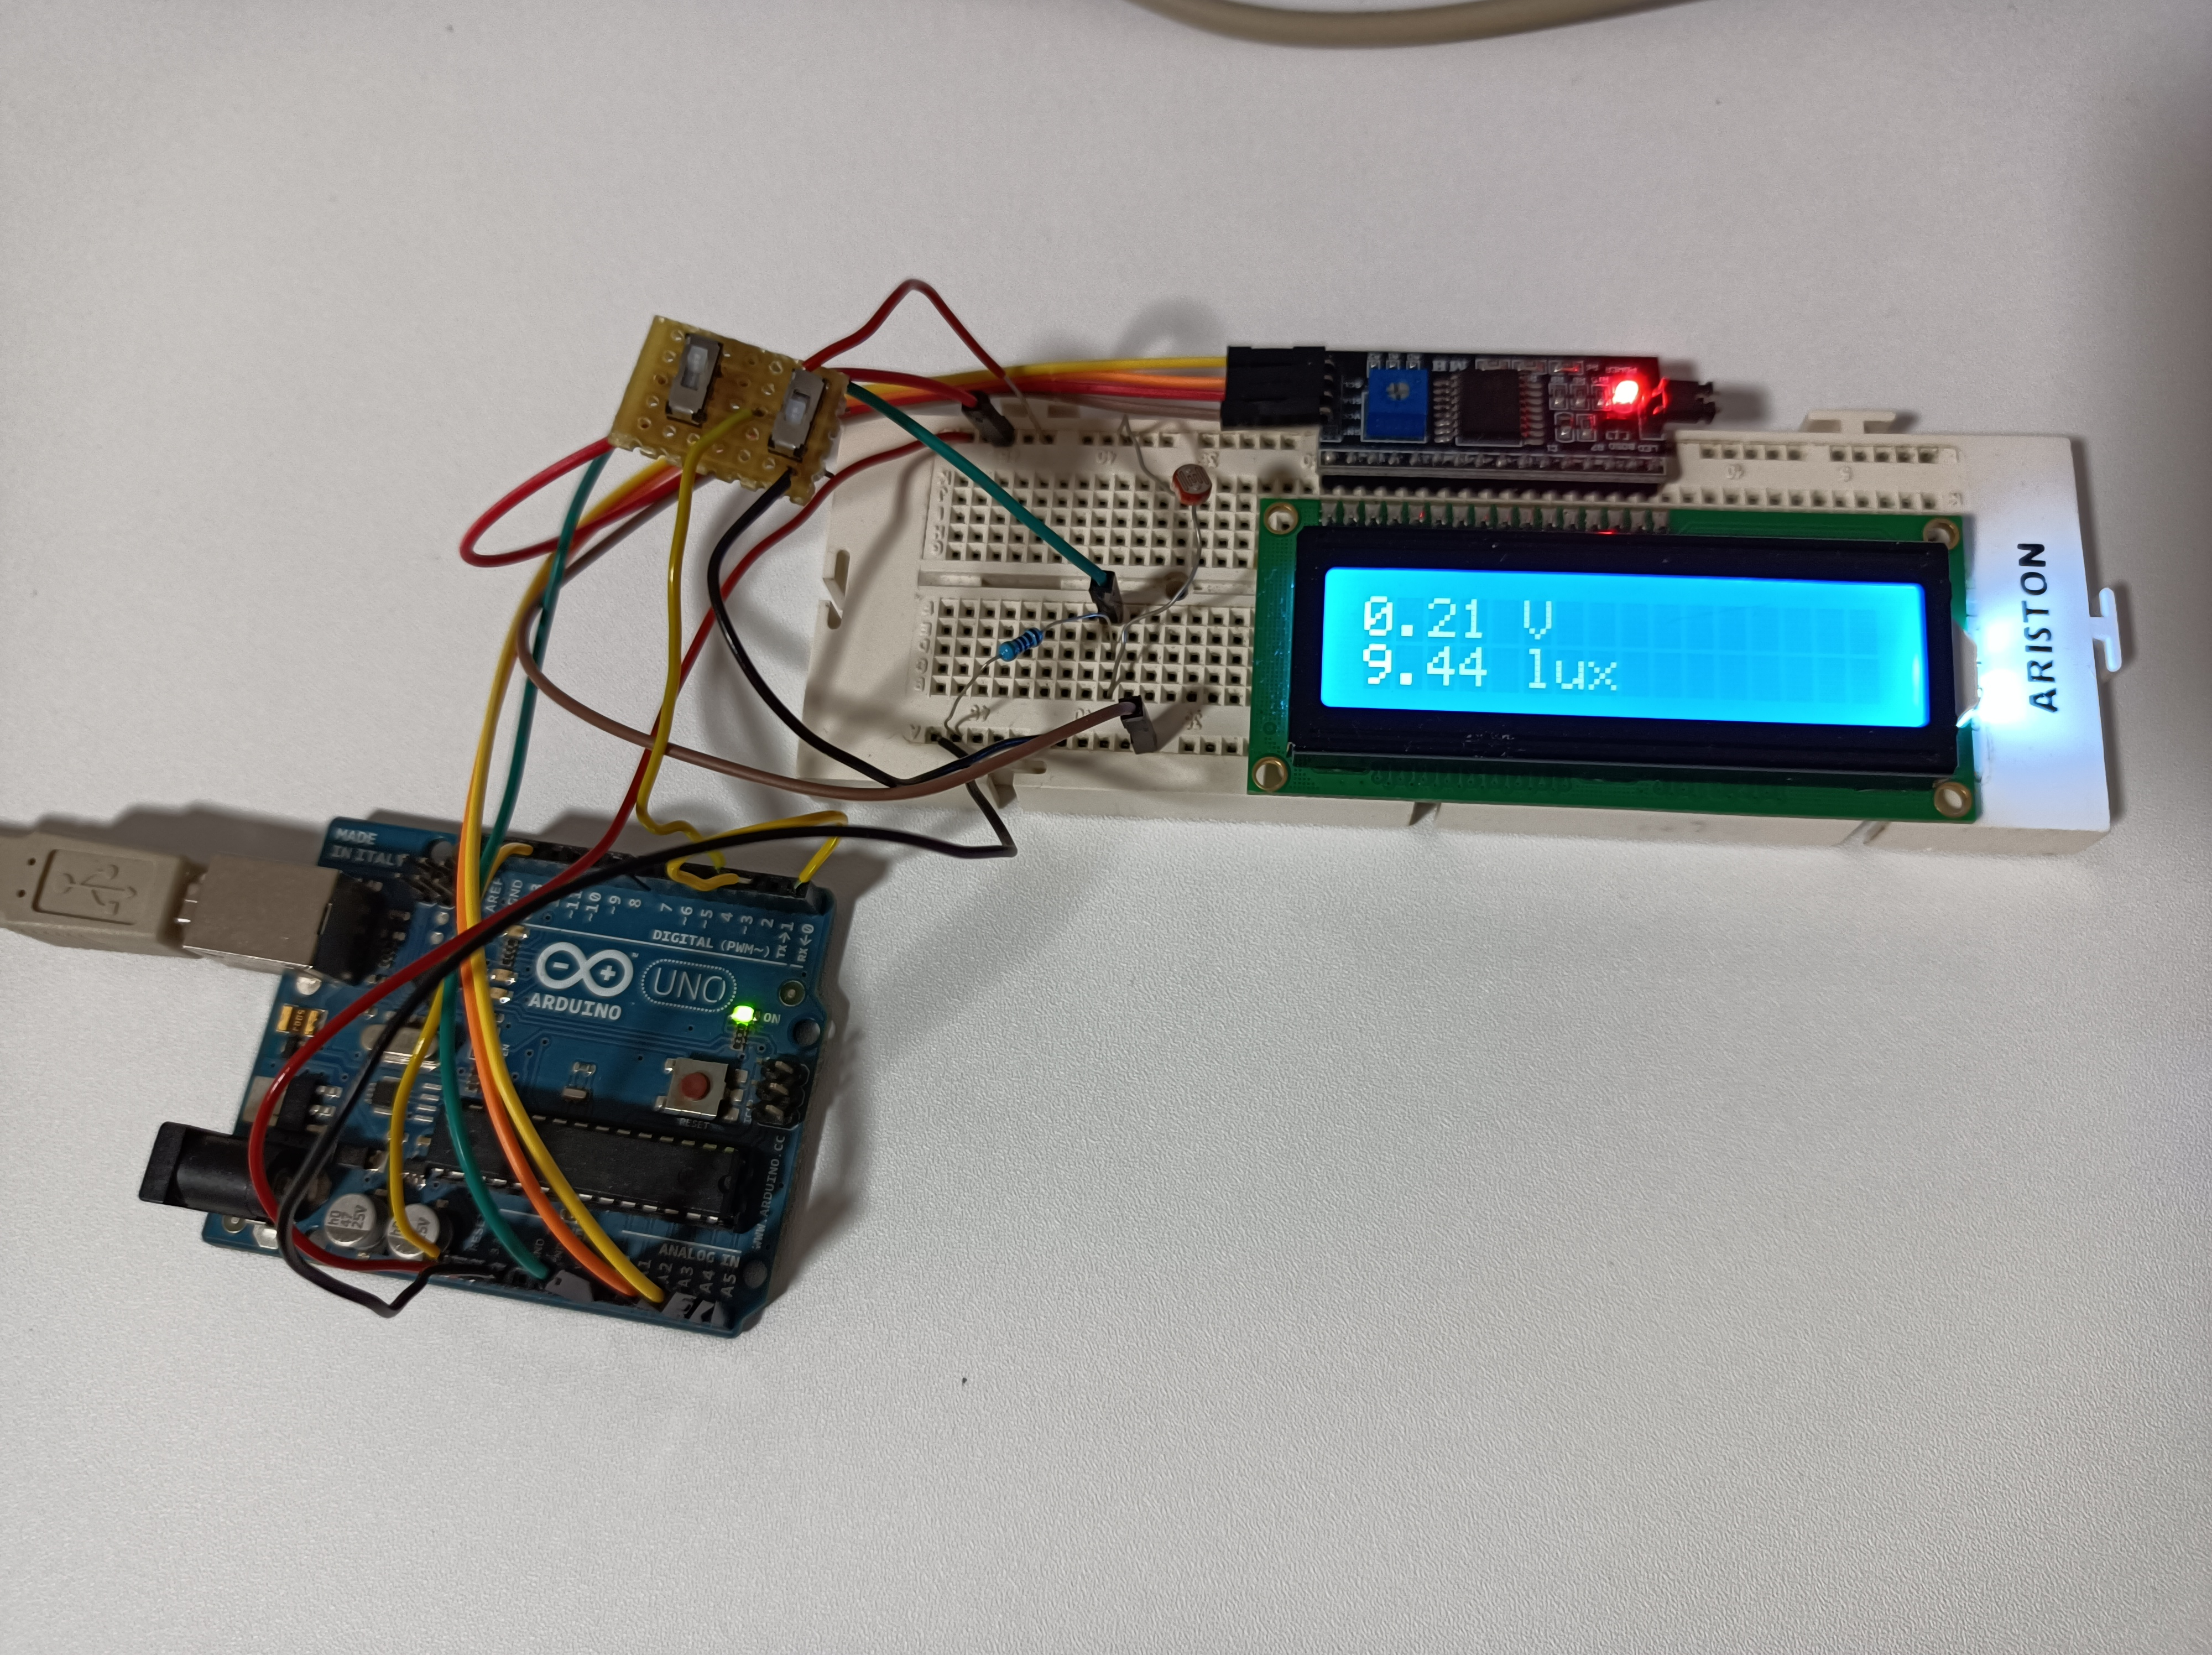
\includegraphics[width=\linewidth]{luxmeter-reader-wiring.jpg}

Para traducir las medidas de resistencia a cifras de luz (lux) con el
fotorresistor usado hay que aplicar la siguiente fórmula:

\begin{equation*}
L = 12518931 \cdot R_l^{-1.405}
\end{equation*}

Donde $L$ es el valor de luz en lux y $R_l$ es el valor de resistencia del
fotorresistor. Éste a su vez debe ser calculado de la siguiente manera:

\begin{gather*}
V_r = \frac{D}{D_{max}} \cdot V_{max} \\
V_l = V_{max} - V_r \\
R_l = \frac{V_l}{V_r} \cdot R_r
\end{gather*}

Donde $D$ es la lectura de valor analógico entre la resistencia y el
fotorresistor, $V_{max}$ la tensión máxima que soporta el pin analógico (que en
este caso son \emph{5 V}), $D_{max}$ la lectura máxima que puede devolver el
puerto (que en este caso es \emph{1023}), $V_r$ es la caída de tensión entre
los terminales de la resistencia, $V_l$ la caída de tensión entre los
terminales del fotorresistor, $R_r$ es el valor de la resistencia fija
(\emph{1 K$\Omega$}) y $R_l$ el valor de resistencia del fotorresistor.

La programación de la placa Arduino se realizaría así teniendo en cuenta estos
procedimientos:

\lstinputlisting[language=C++, caption=luxmeter-reader.ino]{
    1/luxmeter-reader/luxmeter-reader.ino
}

Para la aplicación cliente en el ordenador, creamos un proyecto llamado
\verb|luxmeter-reader| que recibirá las lecturas.

\lstinputlisting[caption=luxmeter-reader/Cargo.toml]{
    1/luxmeter-reader/Cargo.toml
}

\lstinputlisting[language=Rust, caption=luxmeter-reader/src/main.rs]{
    1/luxmeter-reader/src/main.rs
}

\chapter{Raspberry Pi: Preparación}

Instalaremos la distribución Raspbian 10 Lite. Para ello, descargaremos la
imagen recomendada para la práctica\footnotemark. Luego, descomprimiremos el
archivo, lo cual nos dará una imagen que deberemos grabar en una tarjeta SD. En
Linux, esto puede realizarse mediante la siguiente orden desde la terminal
desde el directorio donde se encuentra la imagen, siendo \verb|/dev/sdb| el
nodo de dispositivo correspondiente a la tarjeta:

\footnotetext{\url{
    https://coria.dte.us.es/~bellido/2021-05-07-raspios-buster-armhf-lite.zip
}}

\begin{lstlisting}[language=sh]
sudo dd if=./2021-05-07-raspios-buster-armhf-lite.img of=/dev/sdb bs=4M status=progress
\end{lstlisting}

Podrían usarse otras distribuciones Linux, como Fedora IoT. Sin embargo, el
problema es que el software que instalaremos en ejercicios posteriores
requiere de una interfaz al puerto GPIO obsoleta que no todas las
distribuciones tienen habilitada.

Para habilitar el acceso por SSH desde el primer arranque, colocaremos un
archivo vacío llamado \verb|ssh| (sin extensión) en la raíz de la partición
etiquetada como \verb|boot|. Sin embargo, para que esto sea efectivo sin más,
la conexión a la red deberá ser por cable y sin necesitar adquirir una
dirección IP estática desde el propio dispositivo. Sin embargo, no es este el
caso, dado que usaremos una red WiFi con dirección IP estática. Para configurar
la conexión a la red WiFi adecuada, en nuestro caso con SSID y contraseña
\verb|honeypot| con cifrado WPA personal (WPA-PSK), debemos poner el siguiente
archivo en la raíz de la partición \verb|boot|:

\lstinputlisting[caption=wpa\_supplicant.conf]{
    1/raspberry-pi/wpa_supplicant.conf
}

Para la asignación estática de IP, añadiremos el siguiente texto al final del
archivo \verb|/etc/dhcpcd.conf| en la partición etiquetada \verb|rootfs|:

\lstinputlisting{1/raspberry-pi/dhcpcd.conf}

No se ha usado una conexión cableada dado que ello requeriría el uso de dos
puestos en el aula. Con el método empleado, sin embargo, solo hace falta un
puesto, y en caso de usar un punto de acceso propio (por ejemplo, con el móvil)
ni siquiera se depende del setup del aula.

Al iniciar la Raspberry Pi con la tarjeta insertada, nos conectaremos por SSH
con el usuario \verb|pi| y la contraseña \verb|raspberry| a la dirección IP de
la Raspberry Pi, en nuestro caso \verb|10.42.0.90|. Una vez dentro,
ejecutaremos la herramienta de configuración con permisos de administrador:

\begin{lstlisting}[language=sh]
sudo raspi-config
\end{lstlisting}

Pondremos los siguientes ajustes:

\begin{itemize}
\item \emph{System Options}:
\begin{itemize}
\item \emph{Password}: (cualquiera)
\item \emph{Hostname}: rpi90
\end{itemize}
\item \emph{Interface Options $\rightarrow$ SPI}: Yes
\item \emph{Localisation Options}:
\begin{itemize}
\item \emph{Locale}: es\_ES.UTF-8
\item \emph{Timezone}: Europe, Madrid
\item \emph{WLAN Country}: ES Spain
\end{itemize}
\item \emph{Advanced Options $\rightarrow$ Expand Filesystem}
\end{itemize}

Una vez acabado, cerramos y reiniciamos, tal y como nos pide. Luego volveremos
a ejecutar la herramienta y generaremos el mapa de teclado adecuado yendo a
\emph{Localisation Options $\rightarrow$ Keyboard}.

Finalmente, actualizamos el sistema sin cambiar de versión para recibir mejoras
de seguridad en caso de que existan, reiniciando otra vez tras los cambios:
\begin{lstlisting}[language=sh]
sudo apt-get update -y
sudo apt-get upgrade -y
\end{lstlisting}

\part{Prácticas basadas en MySensors}

\graphicspath{{./2/}}

\chapter{Configuración del gateway y el controlador}

Para instalar el gateway de MySensors, iniciaremos sesión SSH en la Raspberry
Pi y ejecutaremos los siguientes comandos:

\begin{lstlisting}[language=sh]
GIT_COMMIT=093afa0a8a573bda2bb8084b473778795c526532
wget https://github.com/mysensors/MySensors/archive/$GIT_COMMIT.zip -O mysensors.zip
unzip mysensors.zip
cd MySensors-093afa0a8a573bda2bb8084b473778795c526532
./configure --my-transport=rf24 --my-rf24-channel=30 --my-gateway=ethernet --my-port=5003
sudo make install
sudo systemctl enable --now mysgw.service
\end{lstlisting}

Si todo ha ido bien, ejecutaremos la siguiente orden para instalar Domoticz:

\begin{lstlisting}[language=sh]
sudo bash -c "$(curl -sSfL https://install.domoticz.com)"
\end{lstlisting}

Nos preguntará algunos datos. Damos a todo que sí excepto en la carpeta de
instalación, donde indicaremos que sea \verb|/opt/domoticz|.

Podría haberse realizado la instalación con un despliegue conjunto basado en
Docker Compose, pero el problema que presenta este método es que, aparte de
requerir la creación de un recipe personalizado para compilar y empaquetar el
gateway (algo perfectamente realizable), resulta que la comunicación entre
ambos servicios no termina de funcionar aunque se apliquen los ajustes de red
oportunos que se supone que debería tener.

Una vez desplegada la aplicación, abriremos en el navegador el panel de
Domoticz en la dirección \emph{http://<IP>:8080} (en nuestro caso
\emph{http://10.42.0.90:8080}) y configuraremos el idioma y la localización en
el menú \emph{Setup $\rightarrow$ Settings}. De momento dejaremos el usuario y
la contraseña por defecto, que son \emph{admin} y \emph{domoticz}
respectivamente, por lo que no tocaremos nada del cuadro
\emph{Website Protection}, aunque se puede cambiar si así se desea. Una vez
puestos los ajustes necesarios, tal y como aparecen en la siguiente imagen,
pulsaremos \emph{Apply Settings}, lo que nos devolverá a la pantalla de inicio
de sesión. Ahí deberemos introducir las credenciales necesarias.

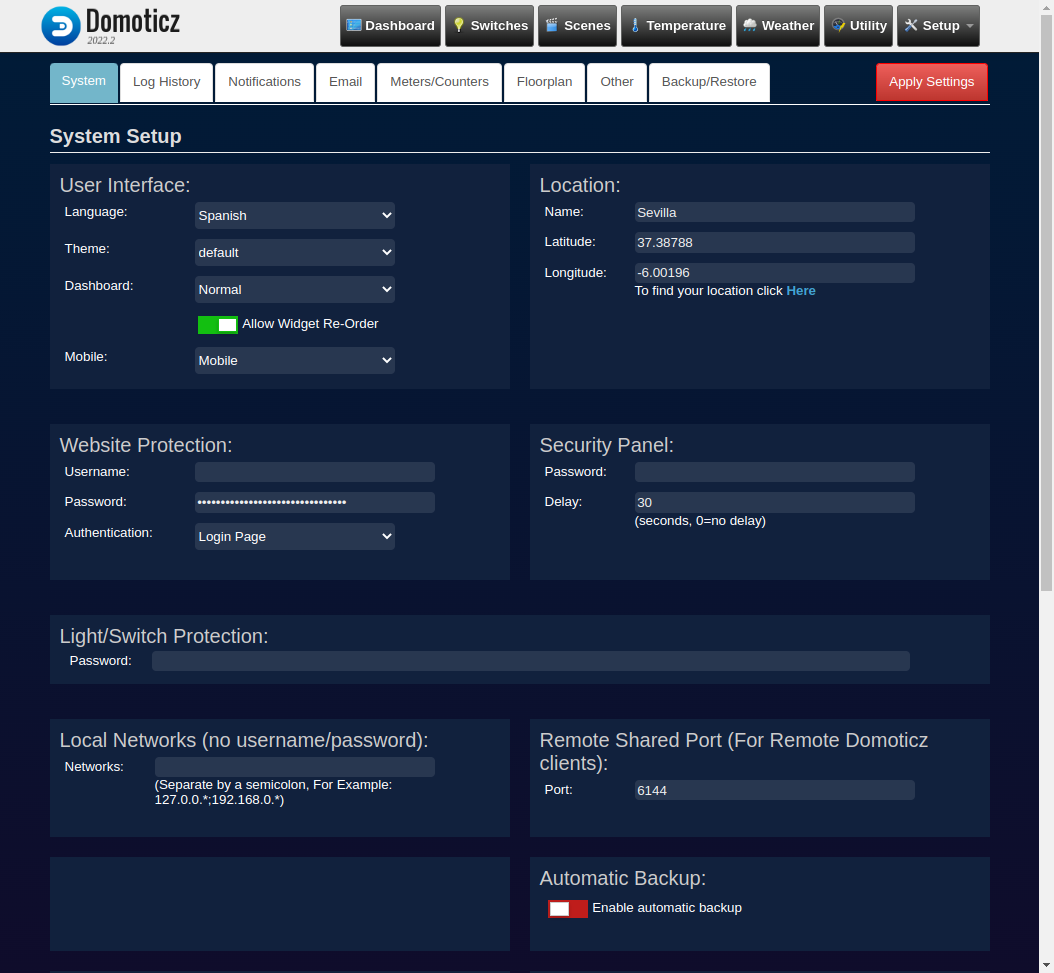
\includegraphics[width=\linewidth]{rpi-setup/domoticz-initial-setup.png}

En \emph{Configuración $\rightarrow$ Hardware}, hay que añadir el gateway de
MySensors con los siguientes parámetros y dándole a \emph{Añadir}:

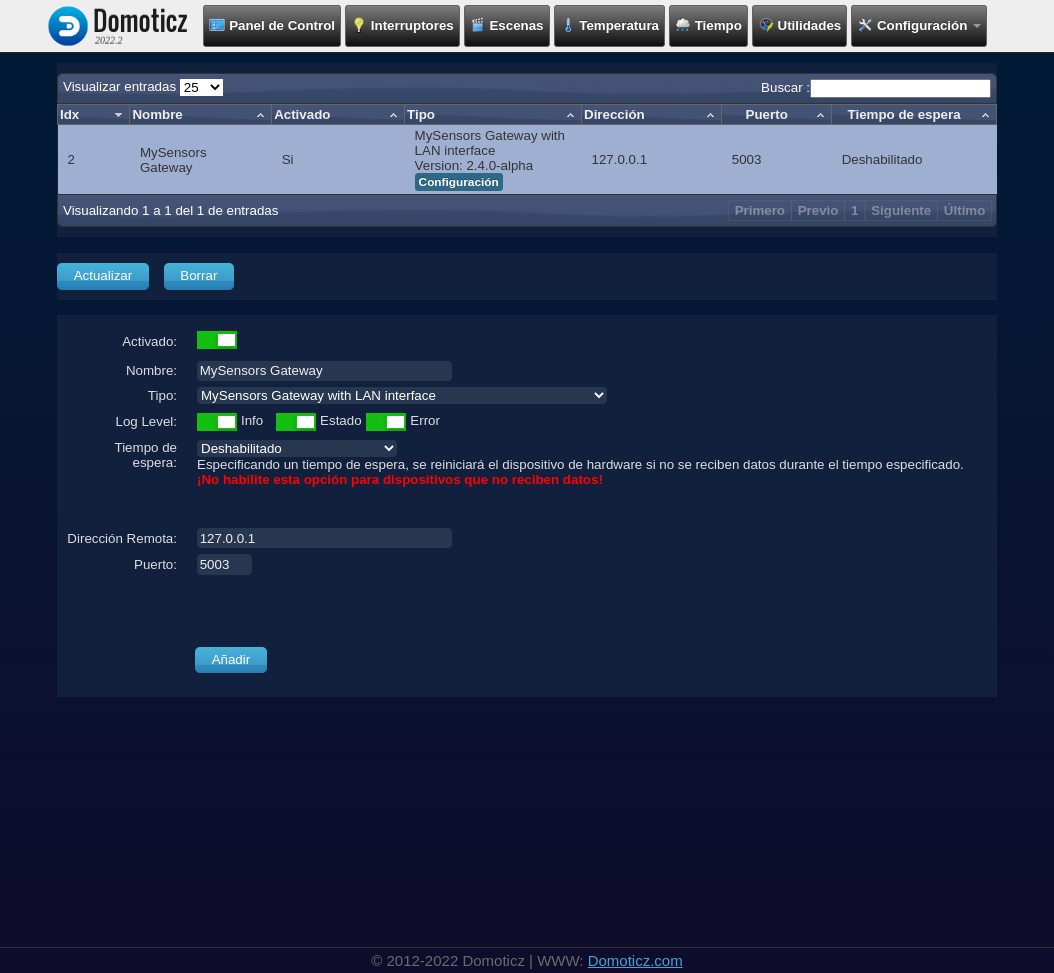
\includegraphics[width=\linewidth]{rpi-setup/domoticz-hardware-setup.png}

En el uso del servicio desde una Raspberry Pi, puede ocurrir que ésta sea
apagada simplemente desconectándola de la alimentación. Esto hace que Domoticz
no se inicie en el siguiente arranque, por lo que hay que reiniciarlo con la
siguiente orden:

\begin{lstlisting}[language=sh]
sudo systemctl restart domoticz
\end{lstlisting}

\chapter{Configuración de la autenticación de mensajes}

Vamos a hacer que la comunicación entre dispositivos de la red de MySensors sea
con autenticación de los mensajes para poder verificar que los mensajes
recibidos son efectivamente del autor que dice ser y que no son falsificados.
Haremos ajustes que dejan el sistema de encriptación preparado también, pero no
lo habilitaremos porque no tiene mucha utilidad, y además puede cargar en
exceso el uso de CPU y RAM de la placa Arduino. La diferencia entre la
autenticación o firma de mensajes y la encriptación es que la segunda se
encarga de ofuscar el contenido de los mensajes, haciéndolo ininteligible a los
receptores externos a la red.

Aún con todo, dependiendo de lo bien que funcione el radiotransmisor y su
alimentación, es posible que de problemas, ya que esta funcionalidad usa el
tamaño máximo en todos los mensajes, sobrecargando en numerosos casos el
transmisor. En tales casos, es conveniente desactivar la función en los nodos.

Lo primero que haremos es generar las claves comunes a todos los dispositivos
del sistema y el identificador del gateway.

El comando en el terminal y la respuesta de generación de la clave HMAC para la
firma de los mensajes es el siguiente:

\begin{lstlisting}[breakatwhitespace=false]
# mysgw --gen-soft-hmac-key 
Generating key... done.
To use the new key, update the value in /etc/mysensors.conf witn:
soft_hmac_key=CBCC9E803E7352556400A9763FE209940A3855937F9496CA5127318B64332771

The next line is intended to be used in SecurityPersonalizer.ino:
#define MY_HMAC_KEY 0XCB,0XCC,0X9E,0X80,0X3E,0X73,0X52,0X55,0X64,0X00,0XA9,0X76,0X3F,0XE2,0X09,0X94,0X0A,0X38,0X55,0X93,0X7F,0X94,0X96,0XCA,0X51,0X27,0X31,0X8B,0X64,0X33,0X27,0X71
\end{lstlisting}

Para la clave AES de cifrado:

\begin{lstlisting}[breakatwhitespace=false]
# mysgw --gen-aes-key
Generating key... done.
To use the new key, update the value in /etc/mysensors.conf witn:
aes_key=96E1E71895239728679998D7FDA3584C

The next line is intended to be used in SecurityPersonalizer.ino:
#define MY_AES_KEY 0X96,0XE1,0XE7,0X18,0X95,0X23,0X97,0X28,0X67,0X99,0X98,0XD7,0XFD,0XA3,0X58,0X4C
\end{lstlisting}

Y el ID serial del gateway:

\begin{lstlisting}[breakatwhitespace=false]
# mysgw --gen-soft-serial 
Generating key... done.
To use the new key, update the value in /etc/mysensors.conf witn:
soft_serial_key=BE60091409F1CE6967

The next line is intended to be used in SecurityPersonalizer.ino:
#define MY_SOFT_SERIAL 0XBE,0X60,0X9,0X14,0X9,0XF1,0XCE,0X69,0X67
\end{lstlisting}

Las claves HMAC y AES deben ser compartidas por todos los dispositivos de la
red domótica, pero el ID serial debe ser único para cada uno.

Para ajustar el gateway con estos datos hay que añadir lo siguiente al final
del archivo \verb|/etc/mysensors.conf|:

\begin{lstlisting}
# Software signing settings
# Note: The gateway must have been built with signing
#       support to use the options below.
#
# To generate a HMAC key run mysgw with: --gen-soft-hmac-key
# copy the new key in the line below and uncomment it.
soft_hmac_key=CBCC9E803E7352556400A9763FE209940A3855937F9496CA5127318B64332771
# To generate a serial key run mysgw with: --gen-soft-serial-key
# copy the new key in the line below and uncomment it.
soft_serial_key=BE60091409F1CE6967

# Encryption settings
# Note: The gateway must have been built with encryption
#       support to use the options below.
#
# To generate a AES key run mysgw with: --gen-aes-key
# copy the new key in the line below and uncomment it.
aes_key=96E1E71895239728679998D7FDA3584C
\end{lstlisting}

Finalmente, para grabar los valores de las claves a la placa Arduino,
descargaremos la carpeta con el personalizador de la seguridad del repositorio
original\footnotemark y pondremos lo siguiente al principio del archivo
\verb|SecurityPersonalizer.ino|, según las claves generadas anteriormente y
generando un ID serial aleatorio:

\footnotetext{\url{
    https://github.com/mysensors/MySensors/tree/093afa0a8a573bda2bb8084b473778795c526532/examples/SecurityPersonalizer
}}

\lstinputlisting[firstline=25, lastline=45, breakatwhitespace=false]{
    2/SecurityPersonalizer/SecurityPersonalizer.ino
}

Cargamos el archivo en la placa Arduino y nos debería marcar al final que la
operación se ha realizado con éxito.

\begin{comment}
+------------------------------------------------------------------------------------+
|                           MySensors security personalizer                          |
+------------------------------------------------------------------------------------+

+------------------------------------------------------------------------------------+
|                               Configuration settings                               |
+------------------------------------------------------------------------------------+
| * Guided personalization/storage of keys in EEPROM                                 |
| * Guided storage and generation of random serial in EEPROM                         |
| * Software based personalization (no ATSHA204A usage whatsoever)                   |
| * Will not require any UART confirmations                                          |
| * Will store HMAC key to EEPROM                                                    |
| * Will store AES key to EEPROM                                                     |
| * Will generate soft serial using software                                         |
| * Will store soft serial to EEPROM                                                 |
+------------------------------------------------------------------------------------+

+------------------------------------------------------------------------------------+
|                           Hardware security peripherals                            |
+--------------+--------------+--------------+------------------------------+--------+
| Device       | Status       | Revision     | Serial number                | Locked |
+--------------+--------------+--------------+------------------------------+--------+
| AVR          | DETECTED     | N/A          | N/A (generation required)    | N/A    |
+--------------+--------------+--------------+------------------------------+--------+

+------------------------------------------------------------------------------------+
|                                   Key generation                                   |
+--------+--------+------------------------------------------------------------------+
| Key ID | Status | Key                                                              |
+--------+--------+------------------------------------------------------------------+
| SERIAL | OK     | B58BDDB48DFD8E2344                                               |
+--------+--------+------------------------------------------------------------------+

+------------------------------------------------------------------------------------+
|                                    Key storage                                     |
+--------+--------+------------------------------------------------------------------+
| Key ID | Status | Key                                                              |
+--------+--------+------------------------------------------------------------------+
| HMAC   | OK     | CBCC9E803E7352556400A9763FE209940A3855937F9496CA5127318B64332771 |
| AES    | OK     | 96E1E71895239728679998D7FDA3584C                                 |
| SERIAL | OK     | B58BDDB48DFD8E2344                                               |
+--------+--------+------------------------------------------------------------------+

+------------------------------------------------------------------------------------+
|                                       EEPROM                                       |
+--------+--------+------------------------------------------------------------------+
| Key ID | Status | Key                                                              |
+--------+--------+------------------------------------------------------------------+
| HMAC   | OK     | CBCC9E803E7352556400A9763FE209940A3855937F9496CA5127318B64332771 |
| AES    | OK     | 96E1E71895239728679998D7FDA3584C                                 |
| SERIAL | OK     | B58BDDB48DFD8E2344                                               |
+--------+--------+------------------------------------------------------------------+

+------------------------------------------------------------------------------------+
|                      This nodes whitelist entry on other nodes                     |
+------------------------------------------------------------------------------------+
{.nodeId = <ID of this node>,.serial = {0xB5,0x8B,0xDD,0xB4,0x8D,0xFD,0x8E,0x23,0x44}}
+------------------------------------------------------------------------------------+

+------------------------------------------------------------------------------------+
|                                  WHAT TO DO NEXT?                                  |
+------------------------------------------------------------------------------------+
| This device has now been personalized. Run this sketch with its current settings   |
| on all the devices in your network that have security enabled.                     |
+------------------------------------------------------------------------------------+

+------------------------------------------------------------------------------------+
|                                  Execution result                                  |
+------------------------------------------------------------------------------------+
| SUCCESS                                                                            |
+------------------------------------------------------------------------------------+
\end{comment}

\chapter{Nodo 1}

Para la construcción del nodo 1, usaremos el siguiente cableado de la placa
Arduino Pro Mini:

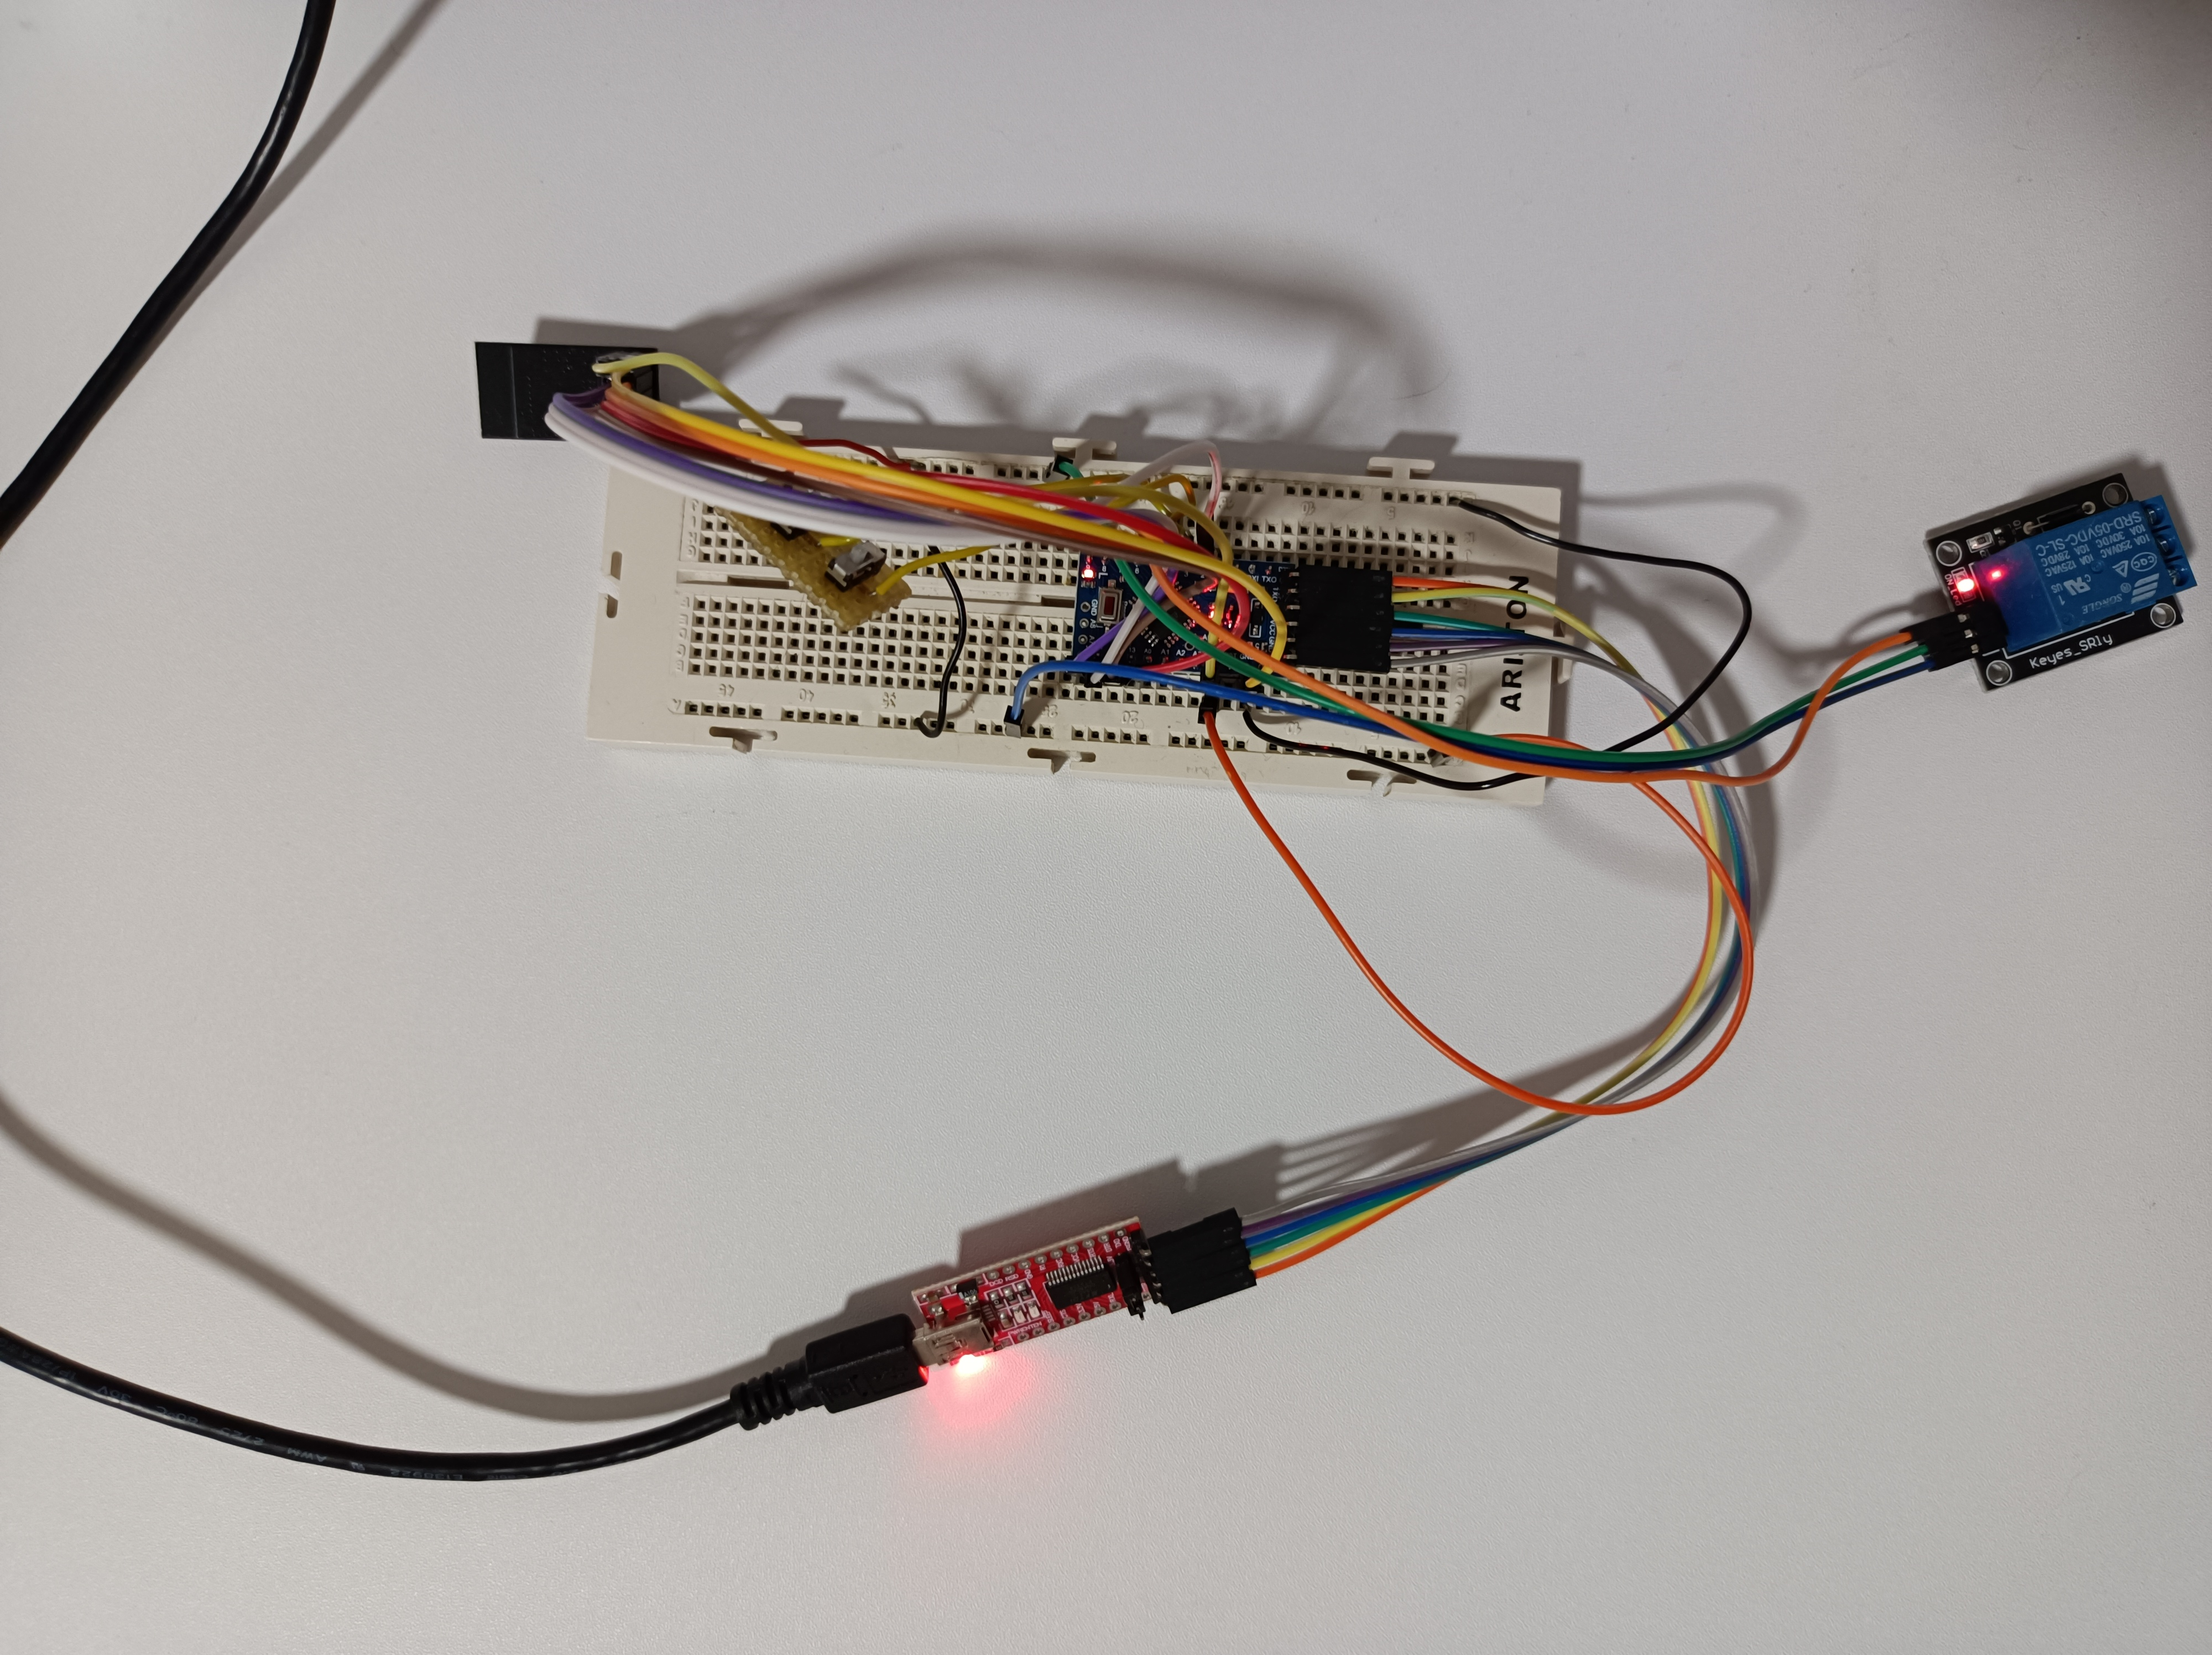
\includegraphics[width=\linewidth]{nodo1/nodo1-wiring.jpg}

La conexión del transmisor de radio NRF24L01 sigue el siguiente esquema:

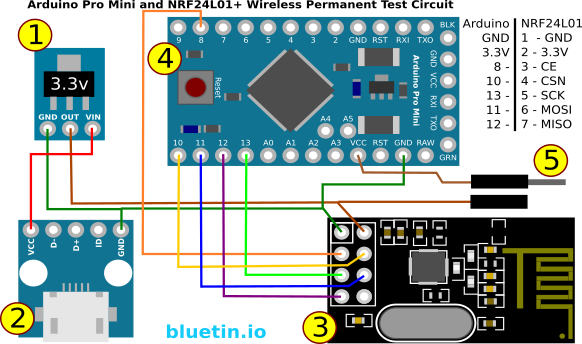
\includegraphics[width=\linewidth]{arduino-nrf24l01-wiring.jpg}

Y a la Raspberry Pi también se le conecta otro transmisor igual:

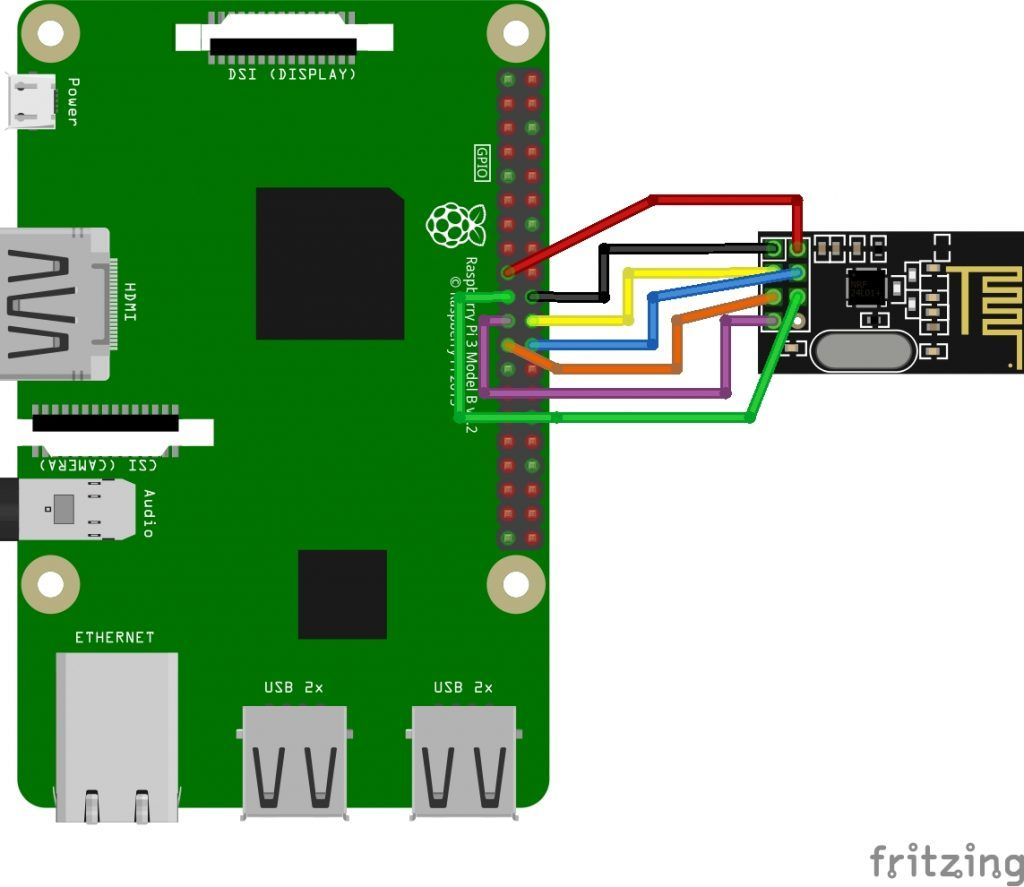
\includegraphics[width=\linewidth]{rpi-nrf24l01-wiring.jpg}

Para la programación de la placa, hay que descargar la librería
\emph{MySensors}, versión \emph{2.3.2}\footnotemark. Para el nodo 1 en
particular, también usaremos la librería \emph{Bounce2}, versión
\emph{2.71.0}\footnotemark.

\footnotetext{\url{
    https://github.com/mysensors/MySensors/archive/refs/tags/2.3.2.zip
}}
\footnotetext{\url{
    https://github.com/thomasfredericks/Bounce2/archive/refs/tags/v2.71.zip
}}

El código que usaremos es el que procede:

\lstinputlisting[language=C++, caption=nodo1.ino]{2/nodo1/nodo1.ino}

Finalmente, en el menú \emph{Configuración $\rightarrow$ Dispositivos} deberían
salir tres entradas como las siguientes, pudiendo activar y desactivar el relé,
que se corresponde con el ID de dispositivo 3:

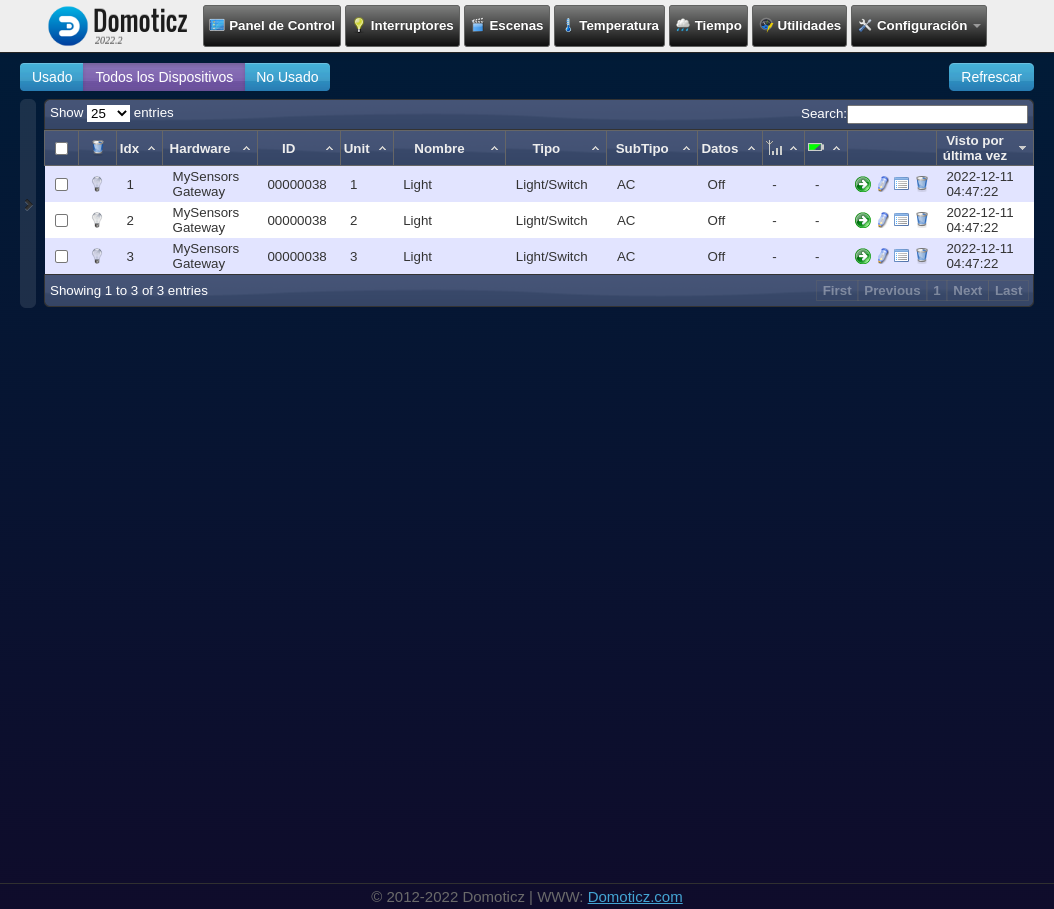
\includegraphics[width=\linewidth]{nodo1/nodo1-domoticz.png}

\chapter{Nodo 2}

\section{Montaje}

Para la construcción del nodo 2, usaremos el siguiente cableado de la placa
Arduino Pro Mini:

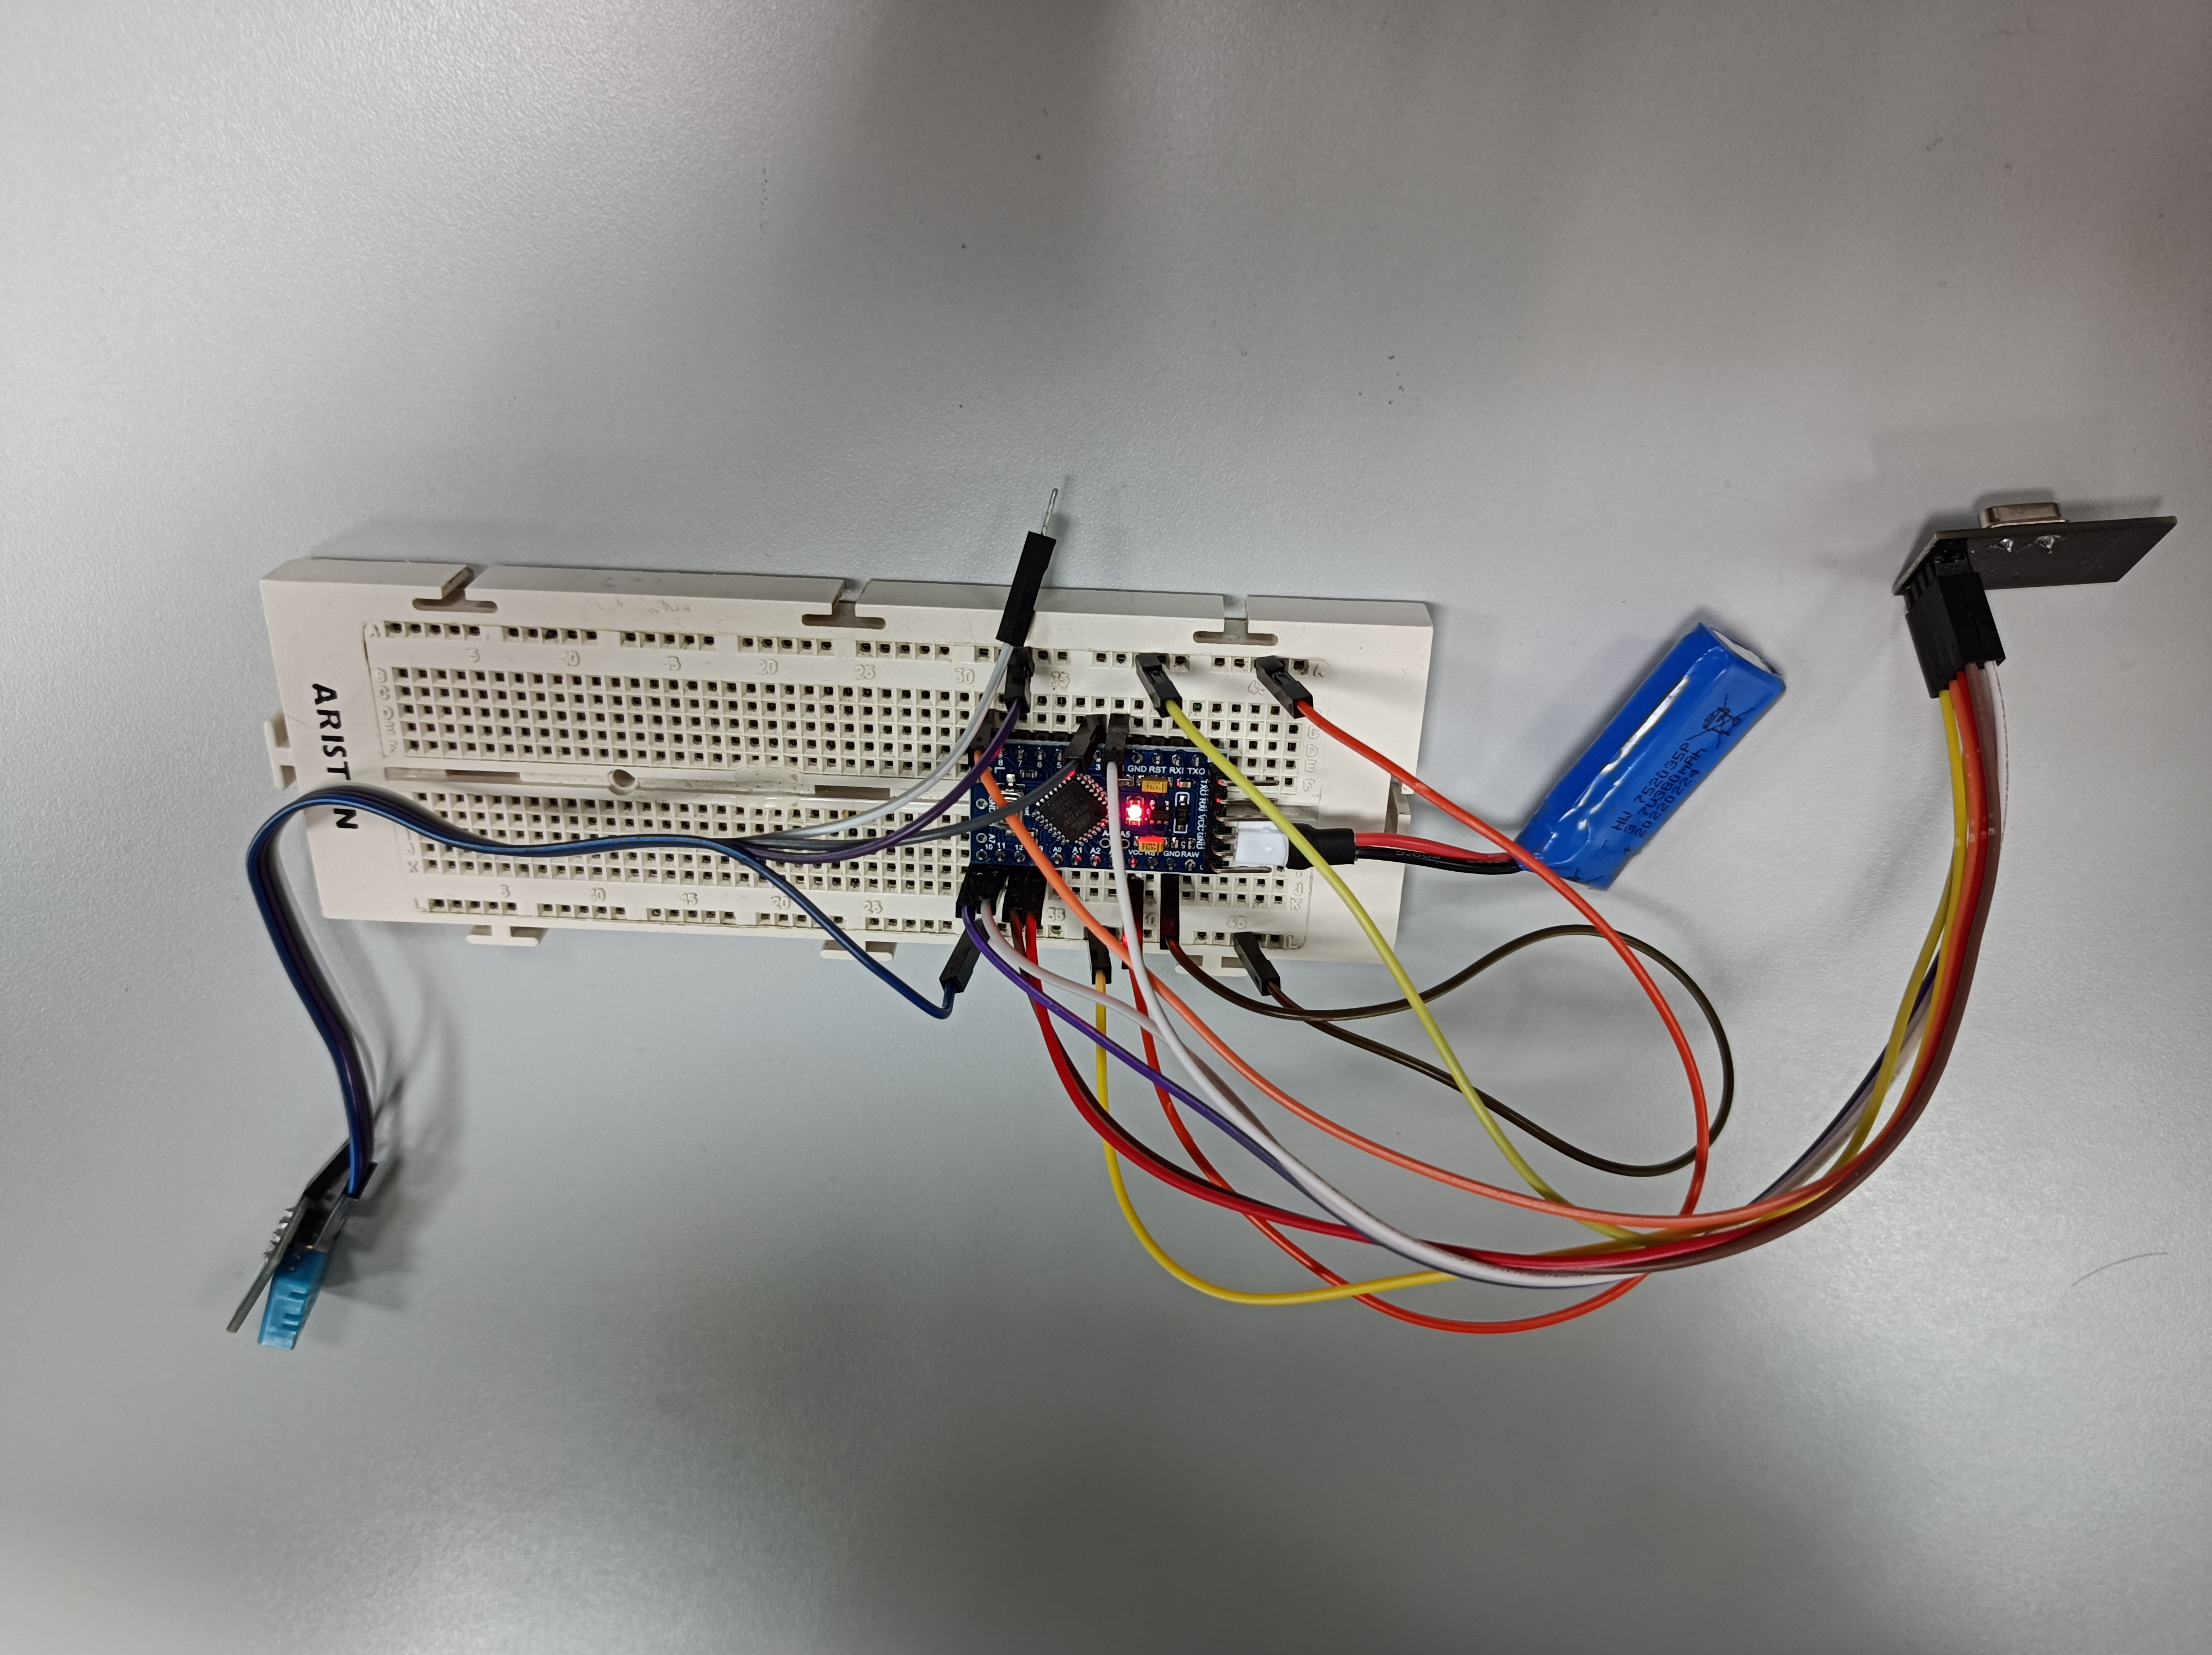
\includegraphics[width=\linewidth]{nodo2/nodo2-wiring.jpg}

Para la programación de la placa, además de la librería \emph{MySensors},
necesitamos las librerías \emph{arduino-DHT}\footnote{\url{
    https://github.com/markruys/arduino-DHT/archive/cd24ce3ca32fe0caf05d6c21565c8d5605860a08.zip
}} y \emph{Arduino\_Vcc}\footnote{\url{
    https://github.com/Yveaux/Arduino_Vcc/archive/2b2362b52e79ce102088c690e2bbcc595563c859.zip
}}.

Usaremos este código:

\lstinputlisting[language=C++, caption=nodo2.ino]{2/nodo2/nodo2.ino}

En este caso, en el menú \emph{Configuración $\rightarrow$ Dispositivos}
debería salir una entrada con las lecturas de temperatura y humedad combinadas,
y la del nivel de batería. También saldrá una lectura adicional de temperatura
que no indica ningún valor, esto es un comportamiento extraño de Domoticz en la
comunicación con MySensors que se desconoce por qué lo hace:

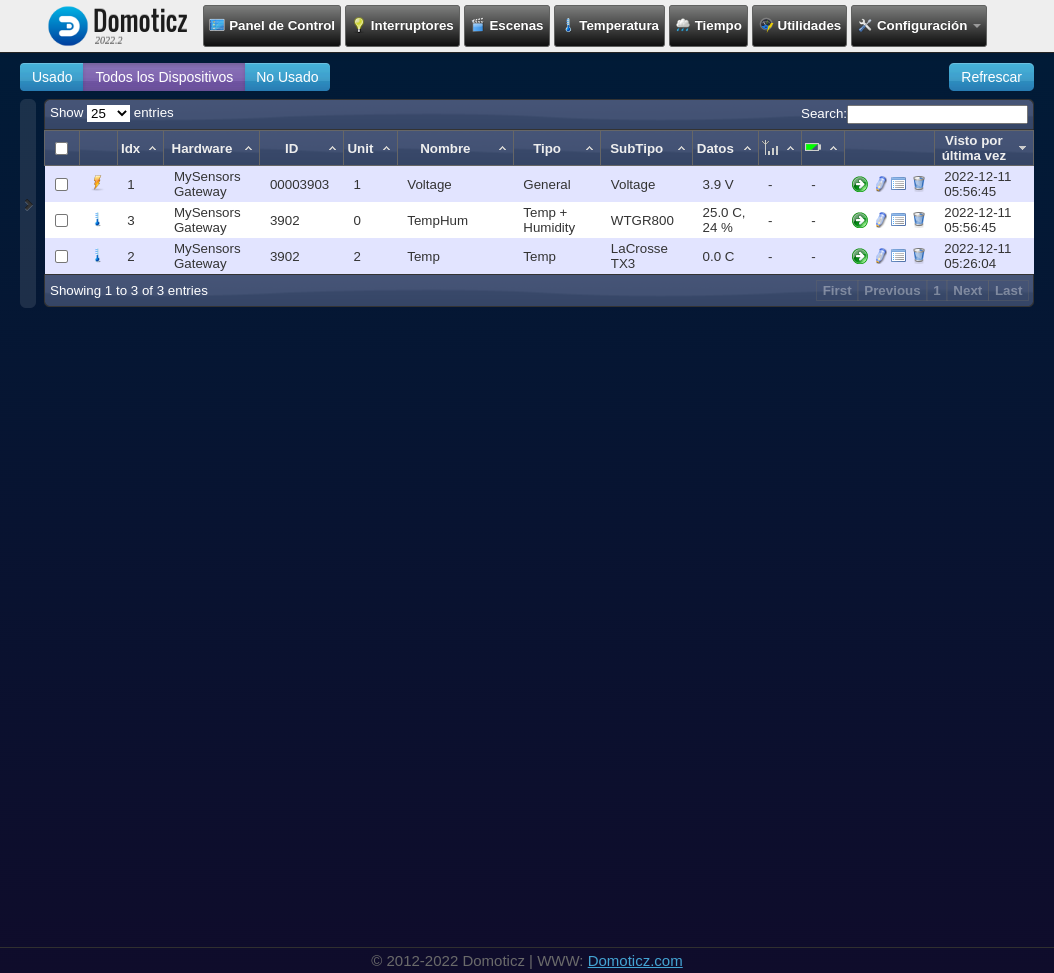
\includegraphics[width=\linewidth]{nodo2/nodo2-domoticz.png}

\section{Medición del consumo}

Para medir el consumo del sistema mientras opera realizaremos el siguiente
montaje. Nótese que la polaridad de la conexión del medidor es la inversa de la
recomendada en el enunciado de la práctica. Esto se hace para evitar lecturas
negativas de intensidad.

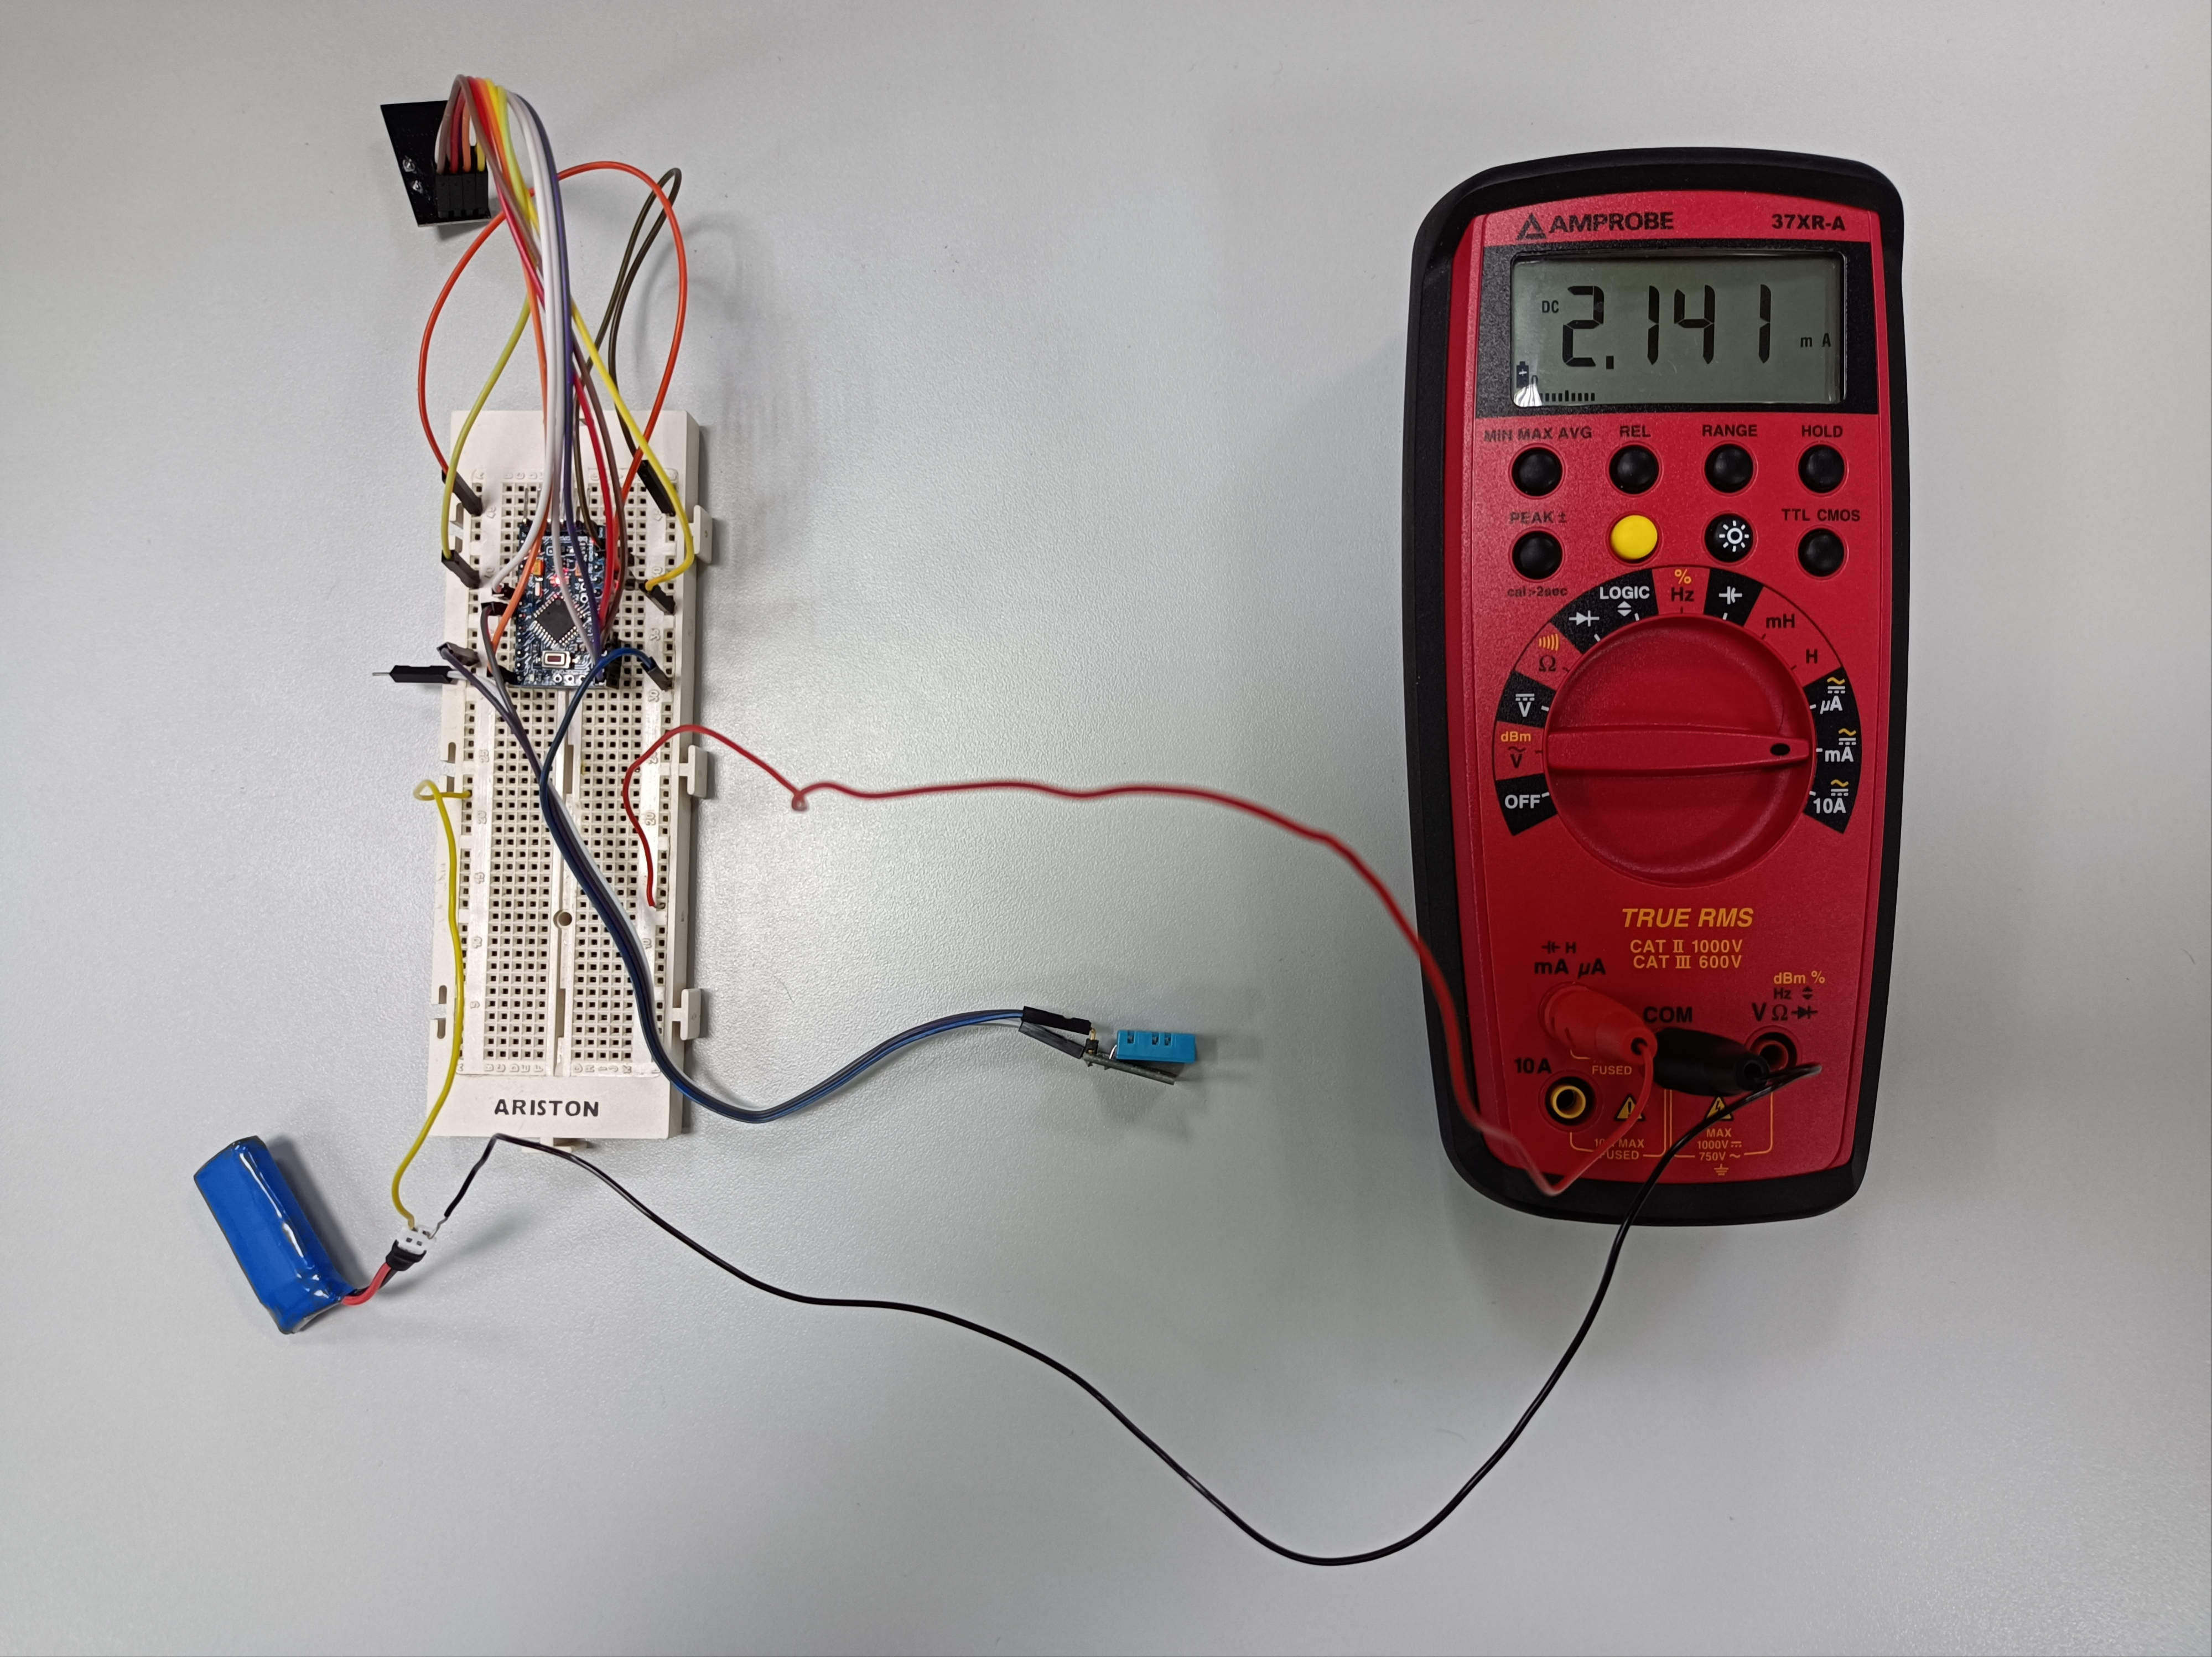
\includegraphics[width=\linewidth]{nodo2/nodo2-consumption.jpg}

La intensidad eléctrica que muestra el medidor es la correspondiente a la
espera entre transmisiones de los valores de medida. Cuando se transmiten datos
este consumo es aproximadamente el doble. Teniendo en cuenta que la tensión de
la batería utilizada era de 3.9 V, entonces el consumo de potencia era de
$2.141\ mA \cdot 3.9\ V \approx 8.35 mW$.

Se sabe que una parte significativa de este consumo base de operación es por el
regulador de tensión incorporado, aunque no se ha realizado la prueba con otra
placa que no lo integre para cuantificar con precisión su impacto.

\part{Diseño y creación de PCBs}

\graphicspath{{./3/}}

\chapter{¿Qué es una PCB?}

\input{3/PCB-intro.tex}

\chapter{Nodo 1 en formato PCB}

\section{Introducción}

En esta práctica vamos a realizar el nodo 1 del bloque 2, pero esta vez las
conexiones entre los dispositivos será fijada de antemano en una PCB, a la cual
se soldarán posteriormente los distintos componentes discretos y conectores
necesarios. Además, no usaremos interruptores físicos para activar el relé,
sino que solo podrá ser manejado desde Domoticz.

Primero empezaremos creando el proyecto desde una de las plantillas estándar,
la correspondiente al Arduino Pro Mini.

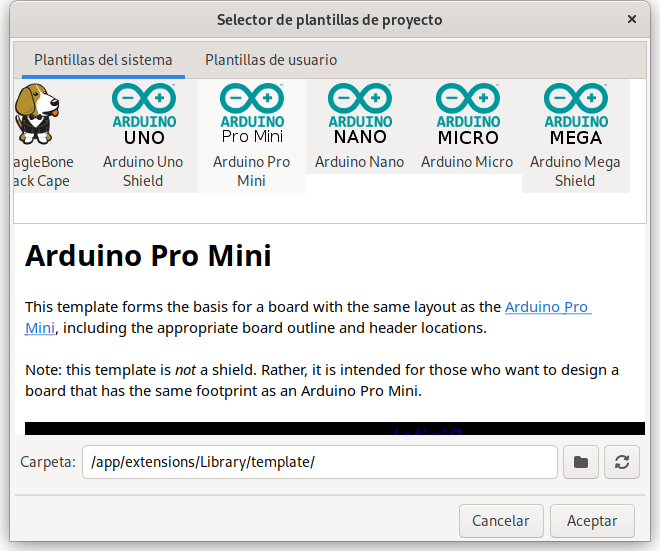
\includegraphics[width=\linewidth]{create-project-template.png}

Luego descargaremos los archivos de símbolo y huella del transistor
BC547C\footnote{\url{
    https://www.snapeda.com/parts/BC547C/ON/view-part/
}} y del relé G3MB-202P\footnote{\url{
    https://www.snapeda.com/parts/G3MB-202P/Omron\%20Automation/view-part/
}} y los descomprimiremos en la carpeta del proyecto de KiCad.

\section{Esquemática}

Abriremos la vista de esquemática haciendo doble click sobre el archivo de
extensión \verb|sch|. Una vez ahí, iremos a
\emph{Preferencias $\rightarrow$ Gestionar librerías de símbolos}, y añadiremos
las siguientes entradas en la pestaña
\emph{Librerías específicas del proyecto}:

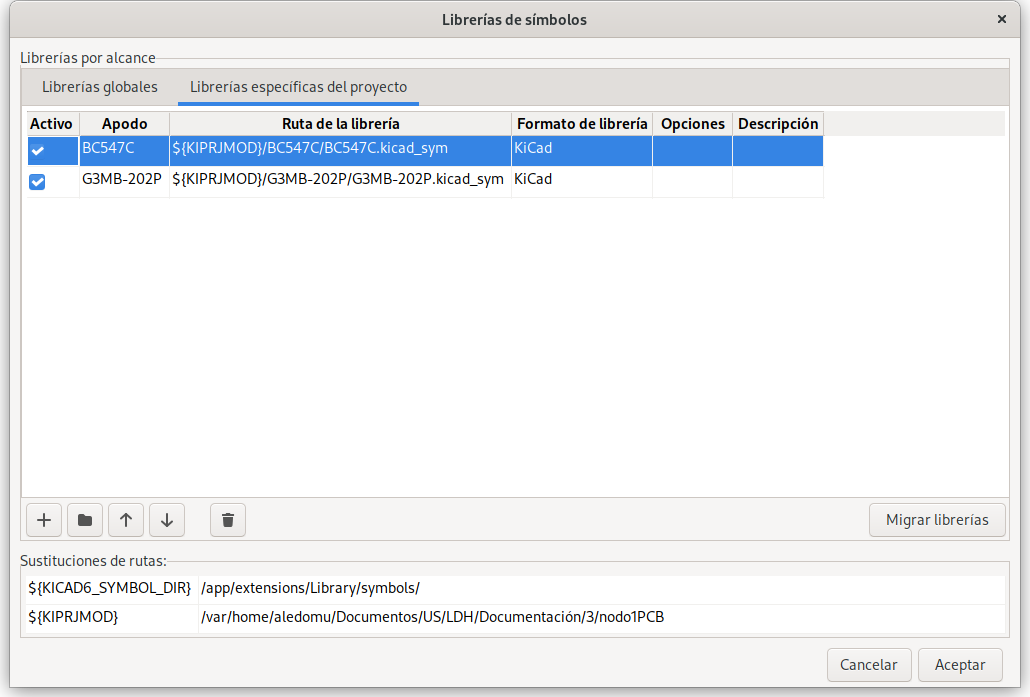
\includegraphics[width=\linewidth]{symbol-path.png}

Una vez importados los símbolos externos necesarios, formaremos la siguiente
esquemática del circuito:

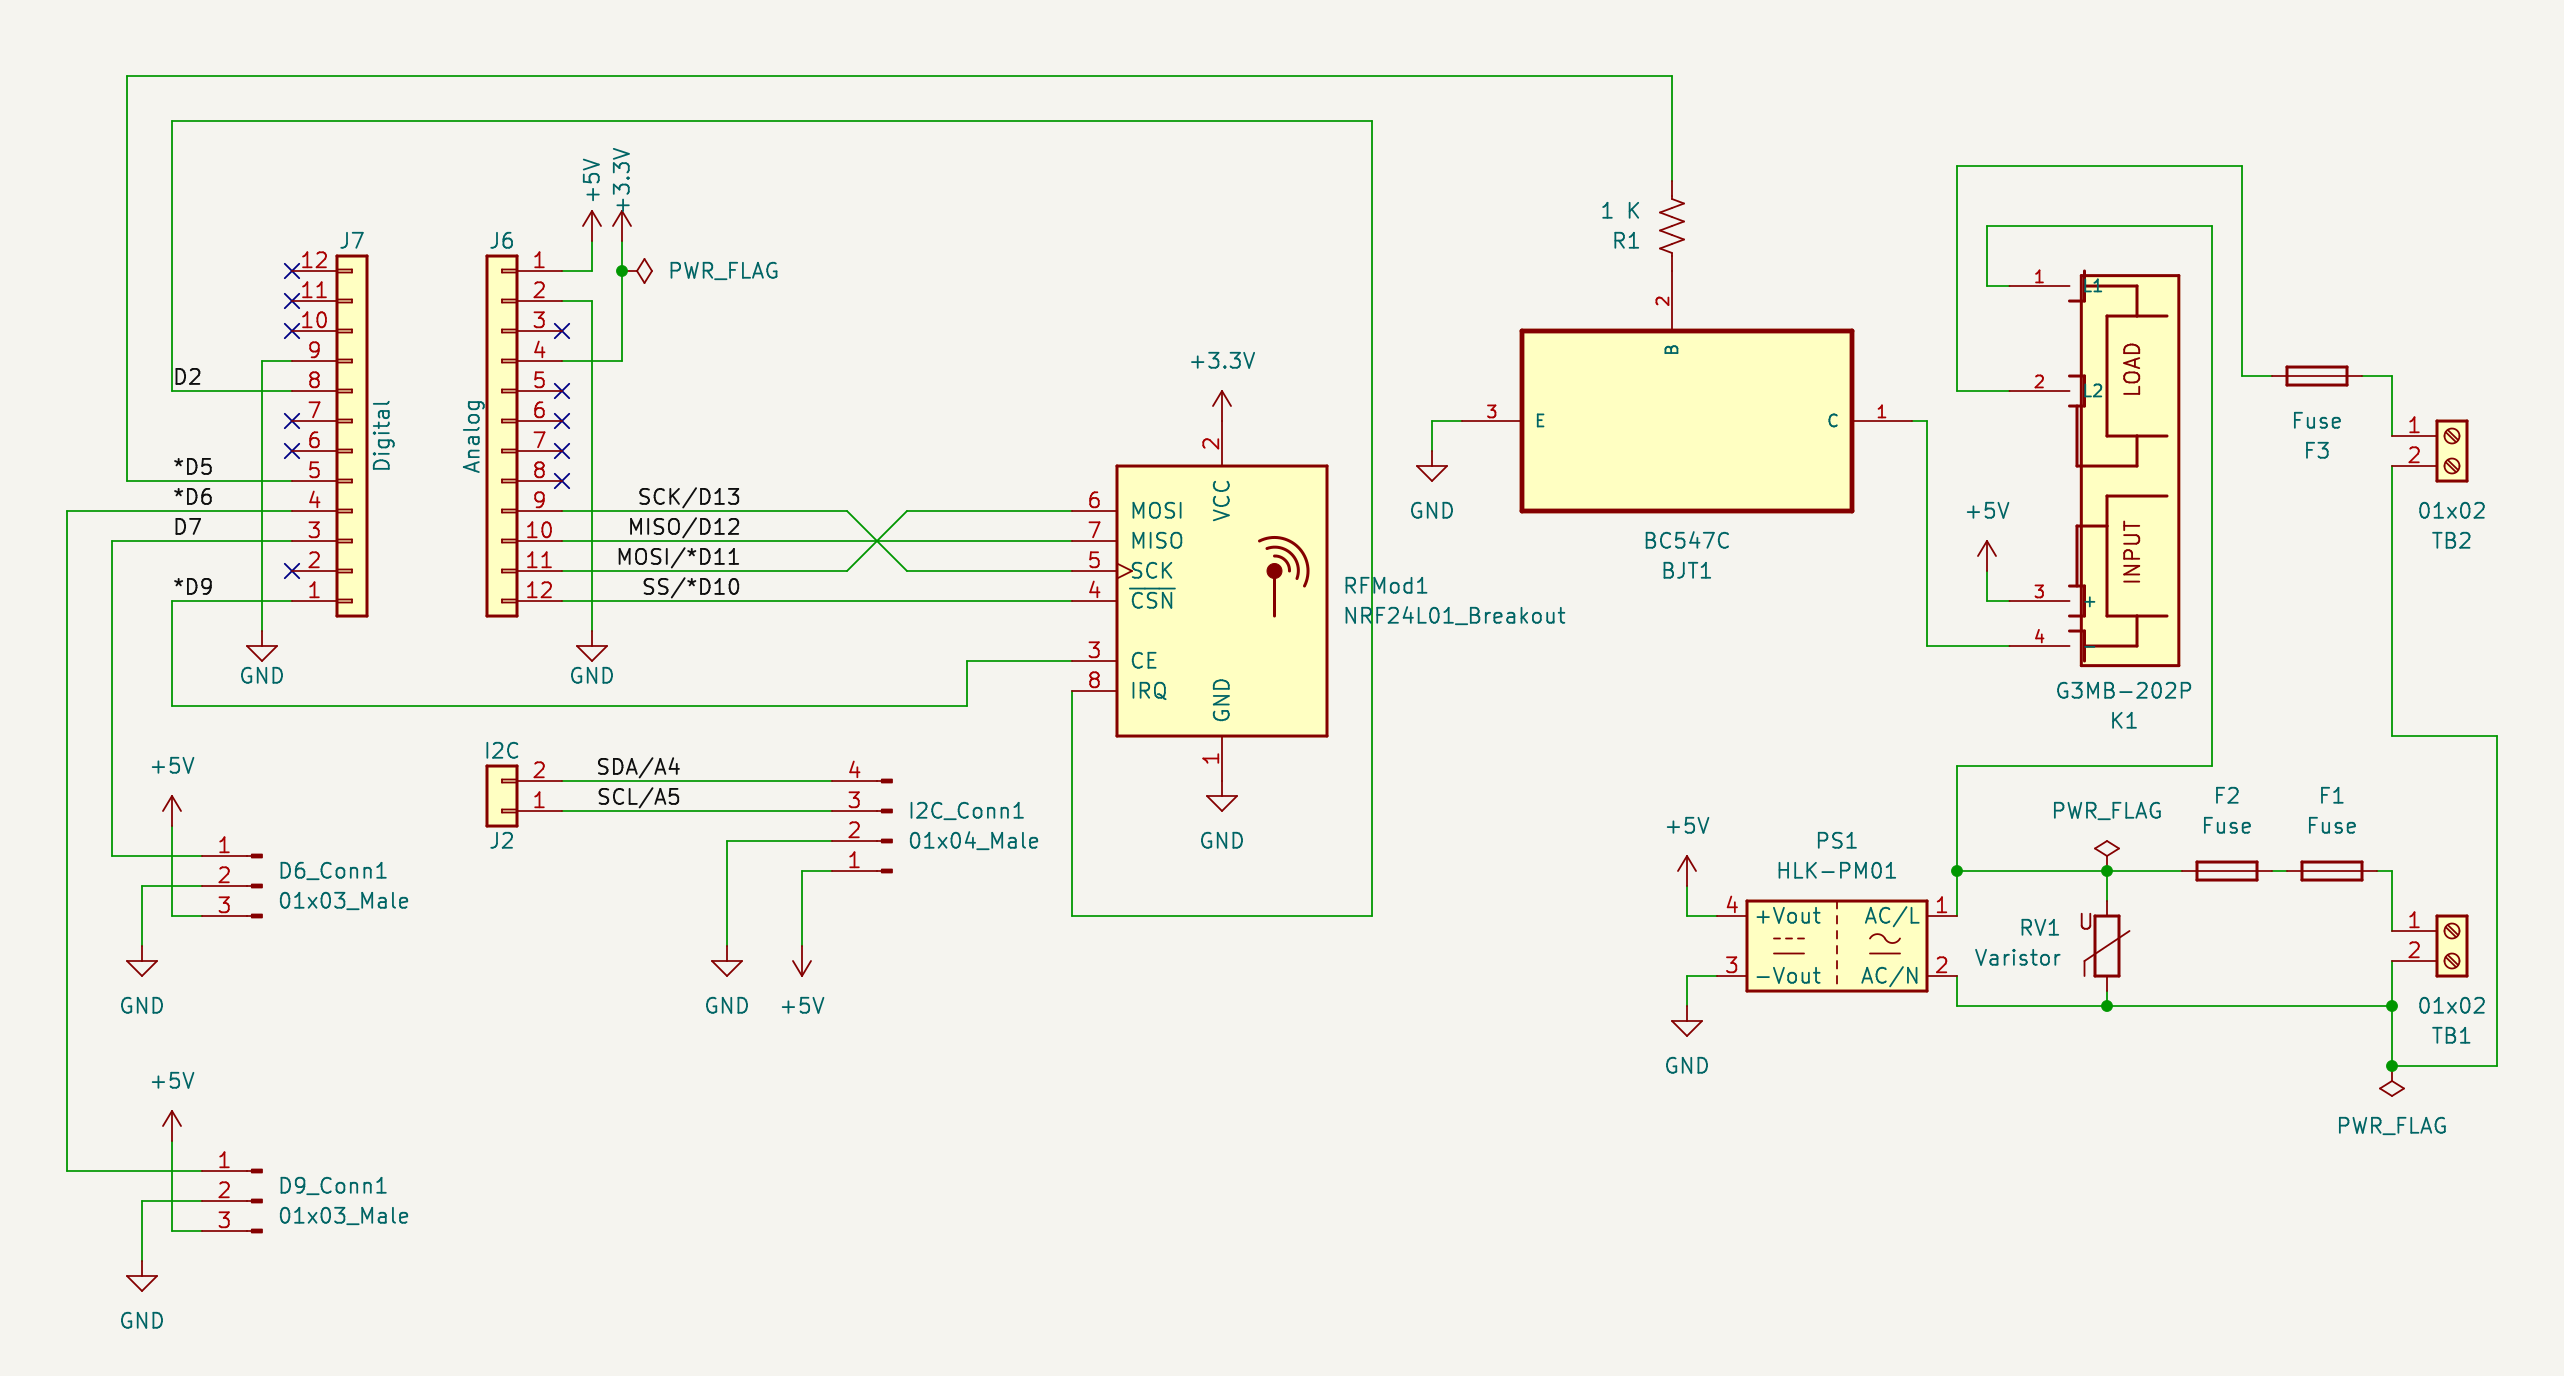
\includegraphics[width=\linewidth]{schematic-general.png}

Nótese que el pin correspondiente a la señal de interrupción del
radiotransmisor está conectado al pin 2 de la placa Arduino.

Finalmente, se deben rellenar los indicadores de referencia de los símbolos de
esquema y comprobar que se cumplen las reglas eléctricas sin un solo error.

\section{Asignación de huellas}

Antes de pasar al diseño de la distribución de los componentes en la PCB,
deberemos ajustar la relación entre componentes y huellas para mantener la
correlación entre la esquemática y el layout. Abriremos la herramienta para
asignar las huellas, en la que primero deberemos importar las huellas
necesarias yendo a
\emph{Preferencias $\rightarrow$ Gestionar librerías de huellas} y añadiendo
las siguientes entradas en la pestaña
\emph{Librerías específicas del proyecto}:

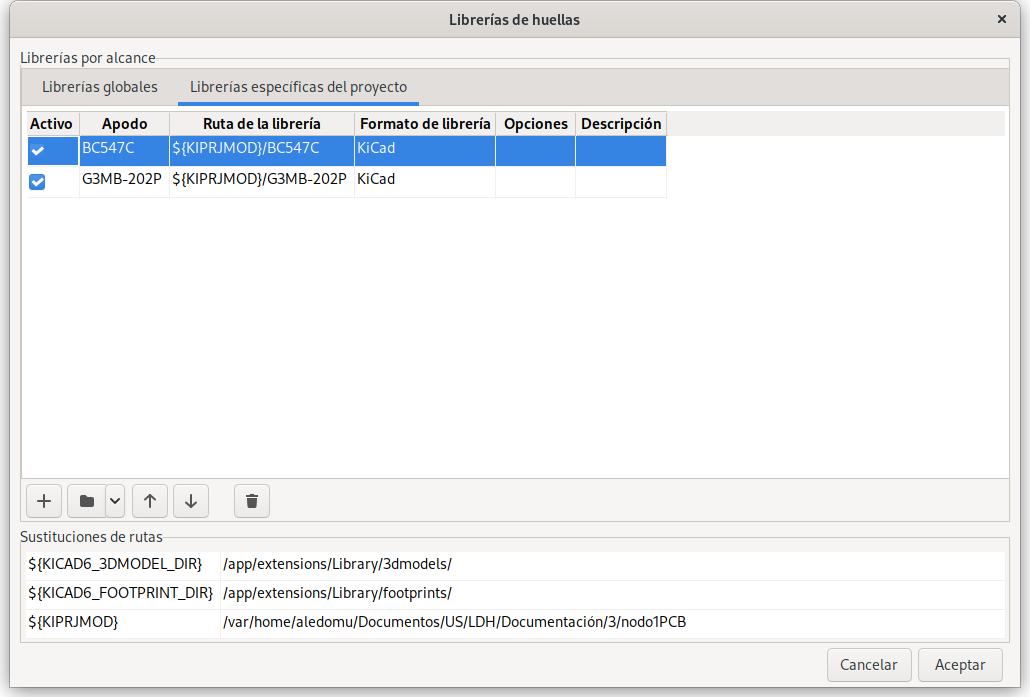
\includegraphics[width=\linewidth]{footprint-path.png}

Una vez importadas las huellas, la asignación que estableceremos es la
siguiente:

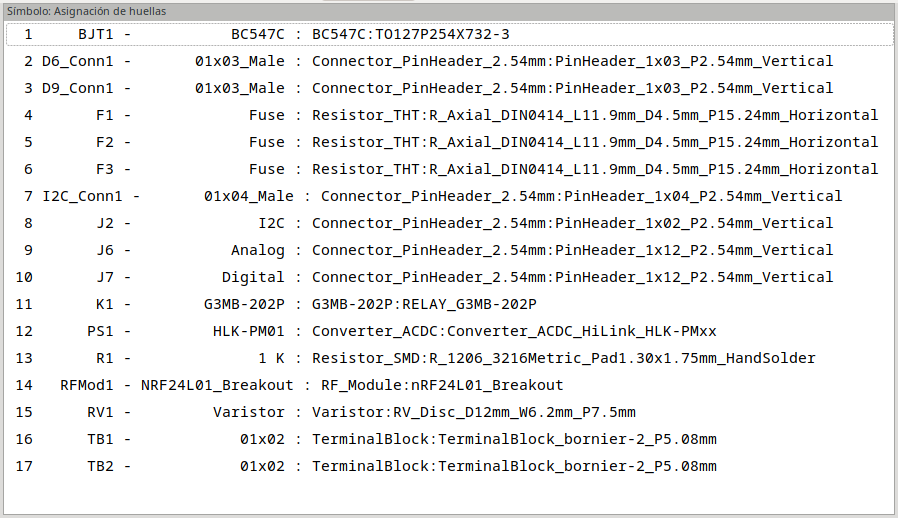
\includegraphics[width=\linewidth]{footprint-assignment.png}

La huella del transistor BJT que se usa es externa, importada anteriormente,
dado que la estándar genera un diseño cuyo resultado da lugar a una PCB en la
que la soldadura del componente es bastante más difícil porque los orificios
están más próximos entre sí.

Ahora sí, desde la vista de esquemática, abrimos la placa en el editor de
placas.

\section{Layout}

En esta fase del diseño de la PCB debemos distribuir espacialmente los
distintos elementos y sus interconexiones, que se realizarán en la capa de
cobre posterior (bottom). Además, como el único resistor que hay en el circuito
se monta de manera superficial (SMD), este hay que cambiarlo de lado en el menú
contextual.

En principio el límite de tamaño con el que contamos es de $10 \times 6$ cm,
pero si se ajusta como se indica en la imagen, se puede reducir a
$9 \times 6$ cm:

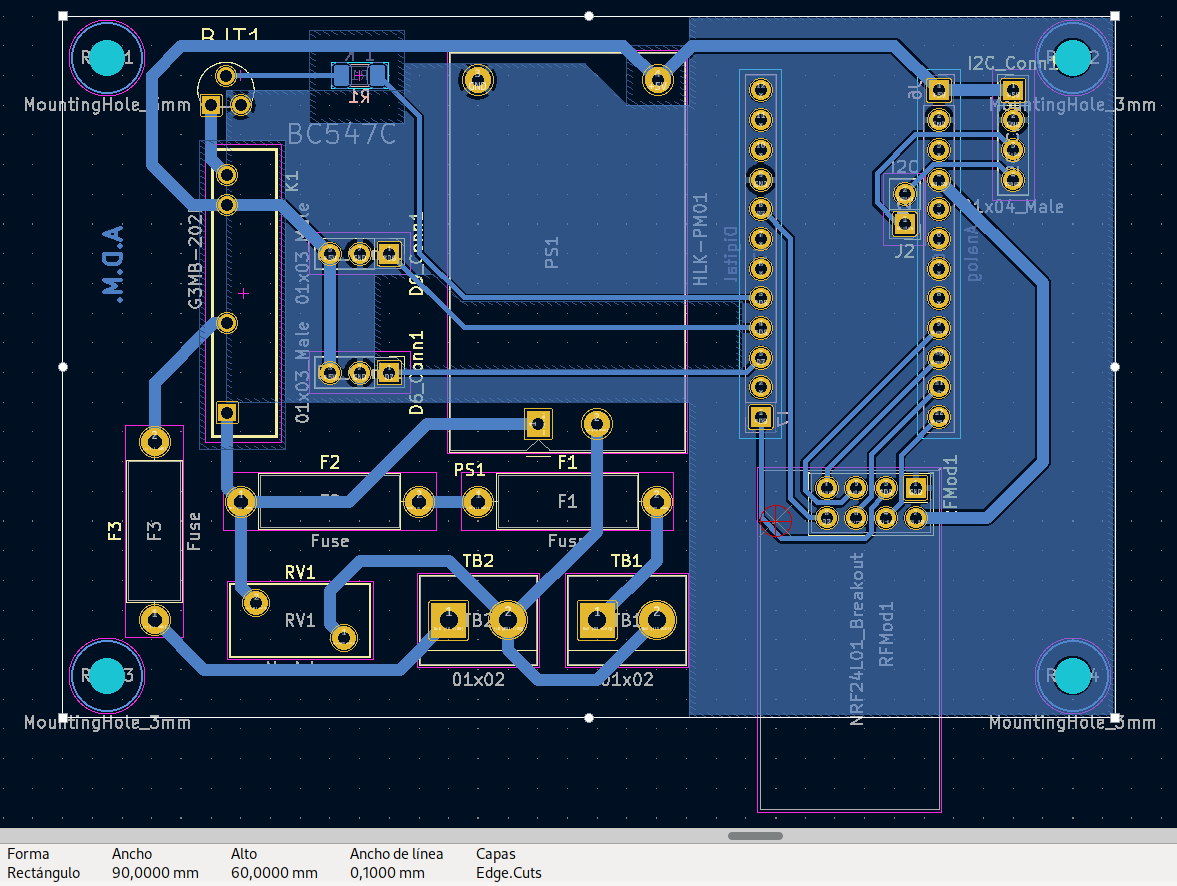
\includegraphics[width=\linewidth]{layout.png}

Las pistas que transmiten señales de alimentación deben tener un grosor de
1 mm, y las que transmiten señales digital deben ser de 0,406 mm. Este último
tamaño no existe de manera predefinida, por lo que se debe editar la lista de
tamaños predefinidos.

La conexión a tierra se establece mediante áreas de cobre que estarán unidasa a
los pads correspondientes a la conexión a tierra de la alimentación en
corriente continua.

Además hay que cambiar el tamaño de los pads del varistor para que el orificio
tenga un tamaño de 1 mm, y el pad en su conjunto de 2 mm. Para ello, hay que
seleccionar ambos e ir a sus propiedades en el menú contextual.

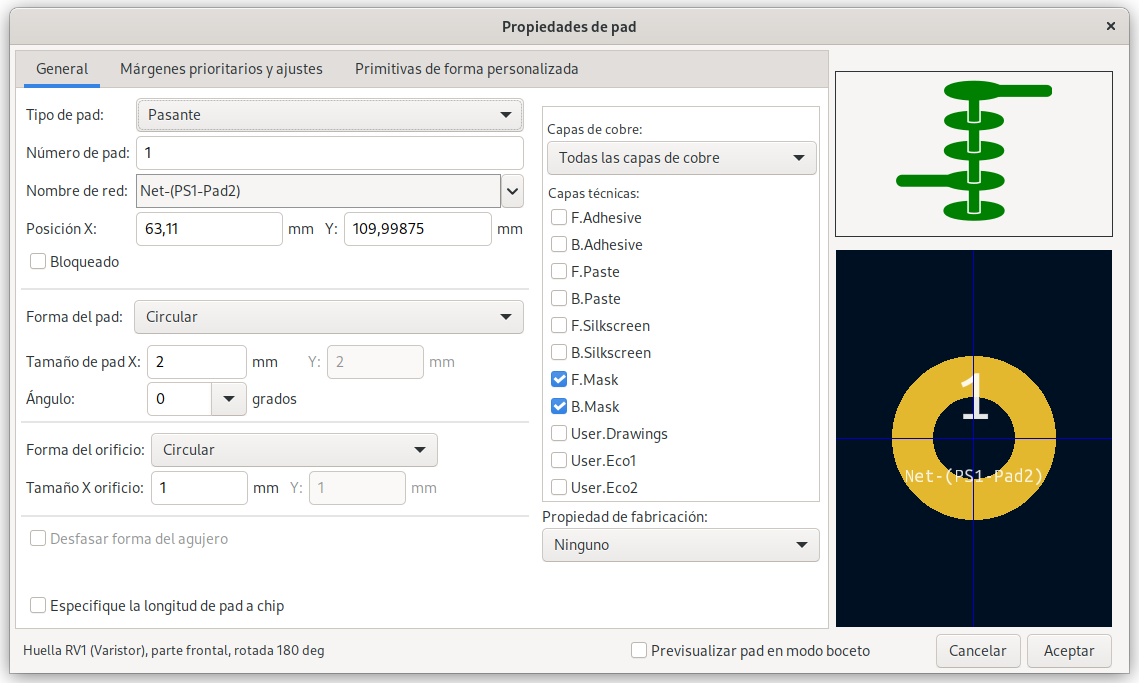
\includegraphics[width=\linewidth]{varistor-pad-hole-size.png}

\section{Trazado}

Una vez acabado el diseño, generaremos los archivos Gerber, necesarios para la
máquina que fabrica la PCB. Para ello iremos a
\emph{Archivo $\rightarrow$ Trazar} y especificaremos los siguientes
parámetros:

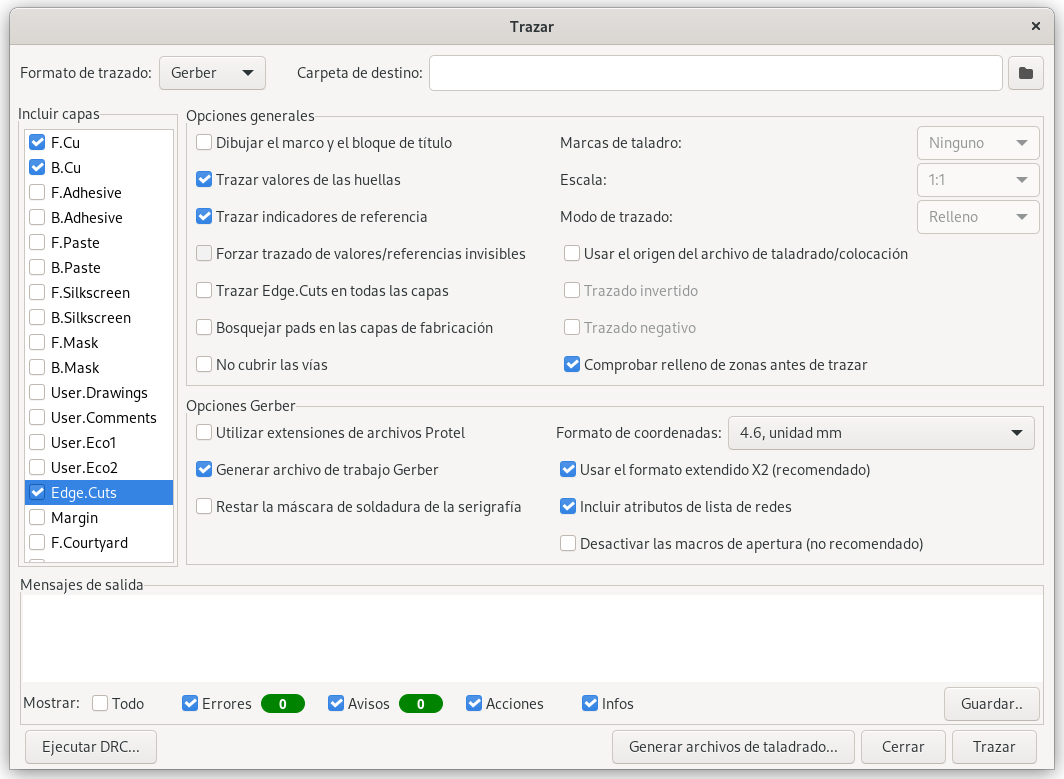
\includegraphics[width=\linewidth]{gerber-file-generation.png}

Primero le damos a \emph{Generar archivos de taladrado}. Nos saldrá otra
ventana, en la que pondremos los siguientes ajustes:

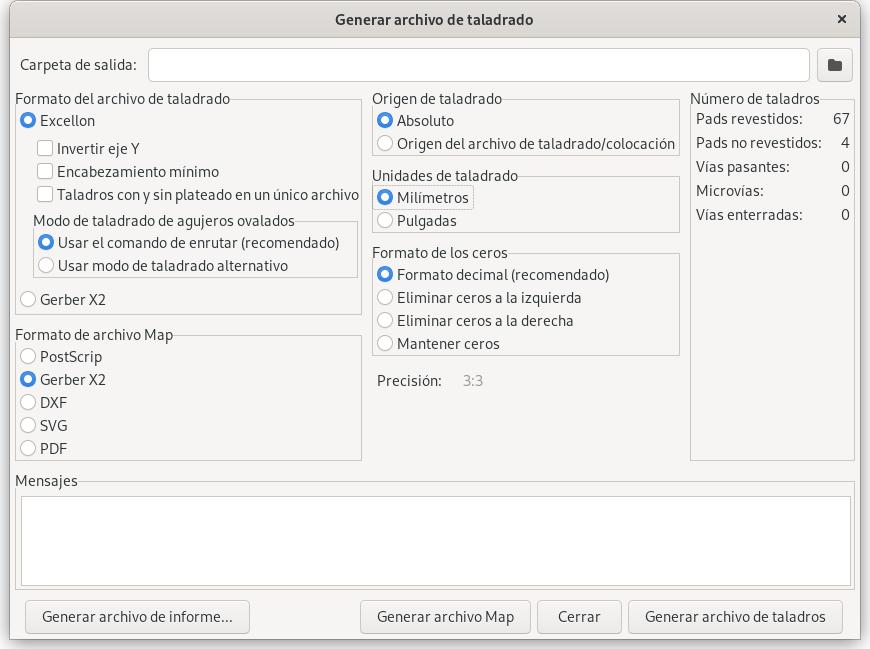
\includegraphics[width=\linewidth]{gerber-drilling-file-generation.png}

Es importante indicar que las unidades de taladrado sean en milímetros para que
los archivos resultantes sean utilizables por la máquina del departamento de la
asignatura, y así poder tener la placa PCB con las especificaciones correctas.

Pulsaremos primero \emph{Generar archivo Map} y luego
\emph{Generar archivo de taladros}. Finalmente, cerramos esta ventana y nos
aparecerá de nuevo la primera, en la que pulsaremos \emph{Trazar}. Deberíamos
tener los archivos correspondientes en la carpeta \verb|output| dentro del
directorio del proyecto.

\section{Análisis del diseño en webs de encargo a fabricación}

Los diseños de PCBs pueden subirse a ciertas páginas web para que expongan
cierta información adicional de los mismos. Para ilustrarlo, usaremos la
utilidad de Eurocircuits\footnote{\url{https://www.eurocircuits.com/}}. Aunque
existen otras, Eurocircuits ofrece un grado de detalle incomparablemente mayor,
por lo que nos limitaremos a esta web.

Eurocircuits permite realizar el pedido inmediatamente una vez hechos los
ajustes pertinentes. Para ello, desde la misma dirección principal, cargaremos
el archivo de layout de KiCad (extensión \verb|pcb|) directamente, dado que
también lo admite además de los gerbers. Podría cargarse también el BOM (Bill
Of Materials), pero no es nuestro objetivo realizar un presupuesto de
ensamblaje completo desde fábrica, así que lo omitiremos.

Para tener un análisis completo, debemos tener una cuenta con la sesión
iniciada y, tras cargar el archivo, añadir la placa al
\emph{carro de la compra} para realizar el análisis completo, el cual tardará
unos minutos. Luego pulsamos en \emph{PCB Visualizer} y veremos los siguientes
datos:

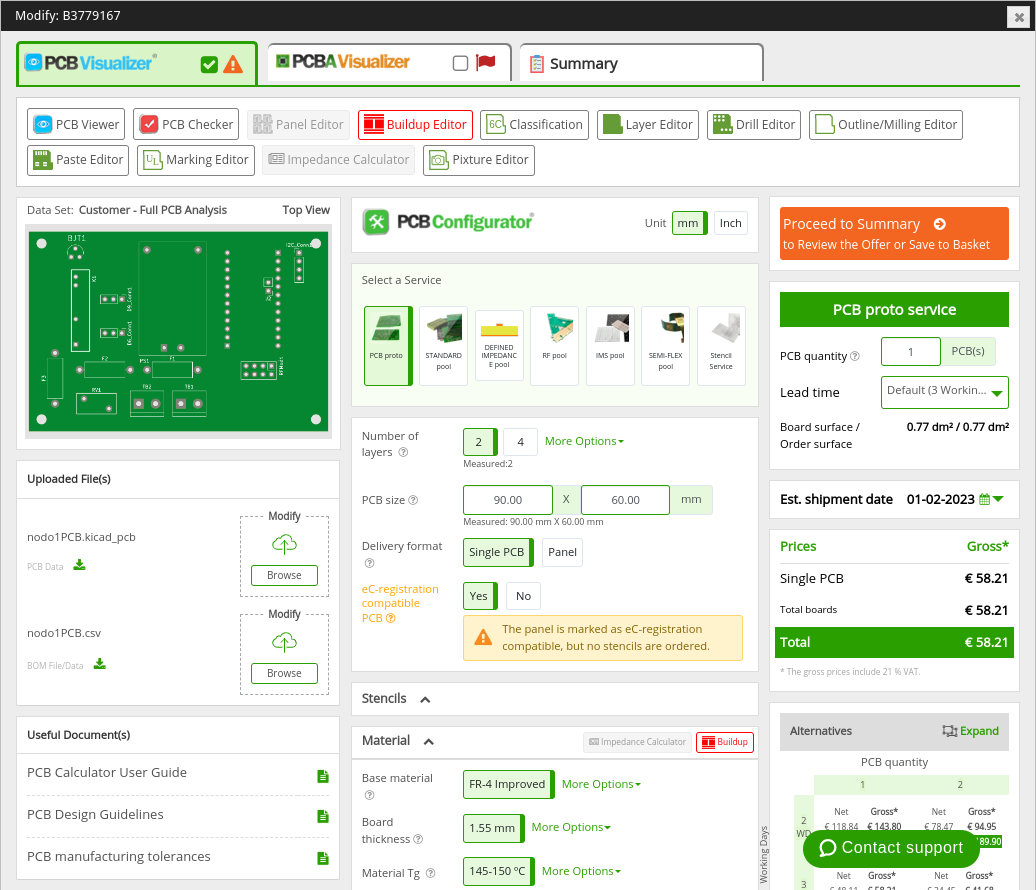
\includegraphics[width=\linewidth]{eurocircuits-pcb-viewer-1.png}

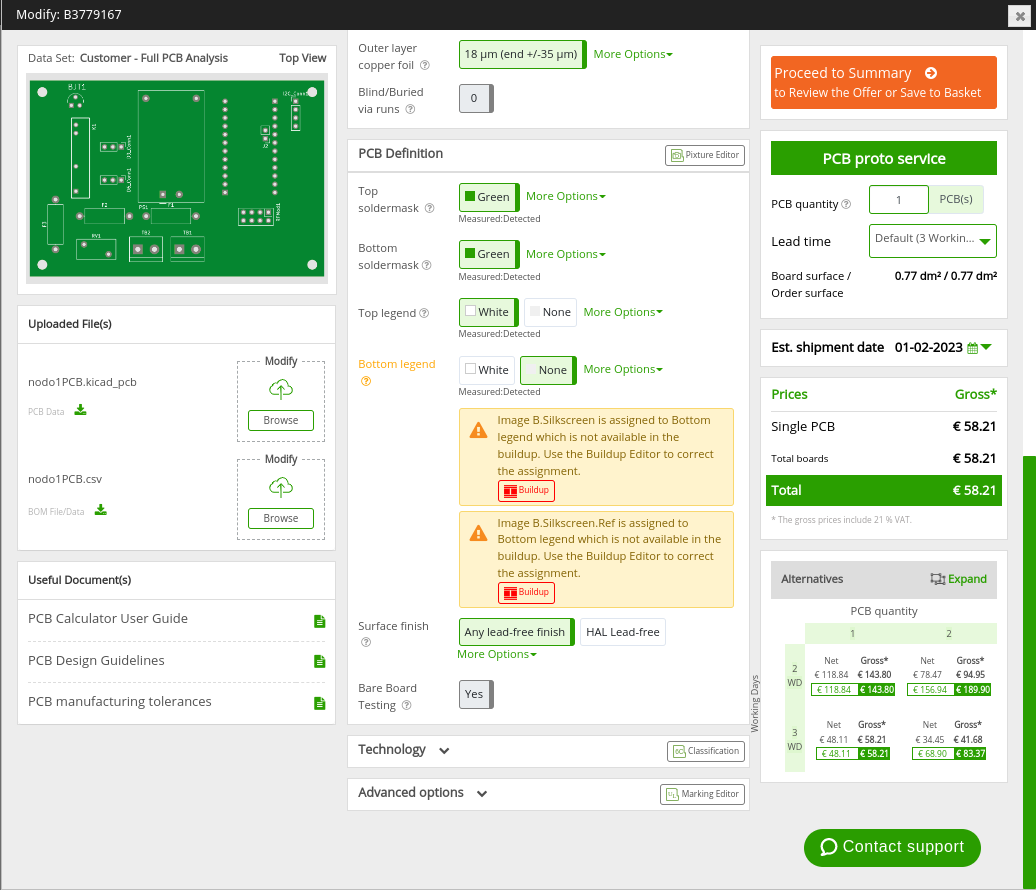
\includegraphics[width=\linewidth]{eurocircuits-pcb-viewer-2.png}

Podemos ver que detecta que la placa tiene dos capas y que su tamaño es de
$9 \times 6$ cm. Además, hay tres advertencias, la primera tiene que ver con
las zonas SMD y las otras dos con la asignación de capas de la leyenda impresa.
La propia herramienta guía de manera relativamente sencilla qué correcciones
hacer.

En base al diseño, también se eligen las opciones más adecuadas. Además, se
pueden realizar ciertas modificaciones. También se puede generar un informe con
la información más importante de la lista de pedidos.

Para usar otras herramientas, hay que generar los archivos gerber de todas las
capas y comprimirlos en un archivo zip. Para ello, hay que repetir los pasos de
la sección de trazado y además seleccionar todas las capas.

\section{Ensamblaje}

El proceso estándar de soldado se realiza poniendo en contacto la punta del
soldador con el terminal del dispositivo colocado en el orificio
correspondiente durante no más de siete segundos a 350 ºC, durante los cuales
se debe también aproximar el hilo de estaño para fundirlo entre la superficie
de cobre, sin exceder los límites de la pista, y el conector terminal.
Previamente hay que colocar fundente en el área, pudiendo ser incluso líquido
depositado con un pincel. La ventilación del lugar debe ser adecuada y hay que
encender un extractor a poca distancia de donde se realice la operación para
evitar inhalar los vapores del fundente y la propia fundición.

En caso de que una soldadura se salga del límite de pista ocasionando una
conexión no deseada, se puede sacar interponiendo una malla de desoldadura
entre la zona y la punta si el exceso es pequeño, disparando una bomba de
desoldar mecánica mientras se refunde el estaño o usando una estación
desoldadora.

Uno de los fusibles es térmico para proteger el circuito de
sobrecalentamientos. El problema de este componente es que la temperatura del
proceso de soldadura puede romperlo, haciendo que deje de conducir. Para
mitigar este riesgo hay que dejar todo el largo a los terminales del fusible,
sin que sobresalga por debajo, y realizar una soldadura a menor temperatura con
muy buen apoyo, con la punta del soldador pegada no más de cuatro segundos.

Los fusibles restantes son de intensidad. Tanto ellos como el varistor pueden
introducirse recortando la longitud de sus terminales al máximo.

Otra particularidad reside en la soldadura del resistor, que se realiza en
superficie. Para que sea exitosa, en lugar de usar un hilo de estaño, se usa
una pasta de estaño entre cada zona de cobre y cada conector del resistor, y se
acerca la punta del soldador caliente directamente, fundiendo la pasta y
pegando el componente a las dos zonas de cobre por separado.

\section{Testado}

Al mismo tiempo que se va realizando el ensamblaje, hay que ir comprobando con
un multímetro que hay conductividad \emph{solo} entre las soldaduras
requeridas. Es imperativo evitar cualquier cortocircuito con masa puesto que
aquí estamos trabajando con tensiones de 220 V. Si hay conductividad donde no
debe haberla, eso significa que alguna soldadura ha excedido los límites de la
pista. Si no hay conductividad donde sí debiera haberla, entonces la soldadura
está demasiado débil y se tiene que terminar.

\section{Programación del Arduino}

El microcontrolador lo cargaremos con el siguiente programa:

\lstinputlisting[language=C++, caption=nodo1PCB.ino]{3/nodo1PCB/nodo1PCB.ino}

Aquí estamos reutilizando la configuración de autenticación y/o encriptado que
haya sido usada en el bloque 2, junto con la del gateway en la Raspberry Pi.

\section{Resultado}

Tras soldar todos los componentes, la PCB debería quedar así:

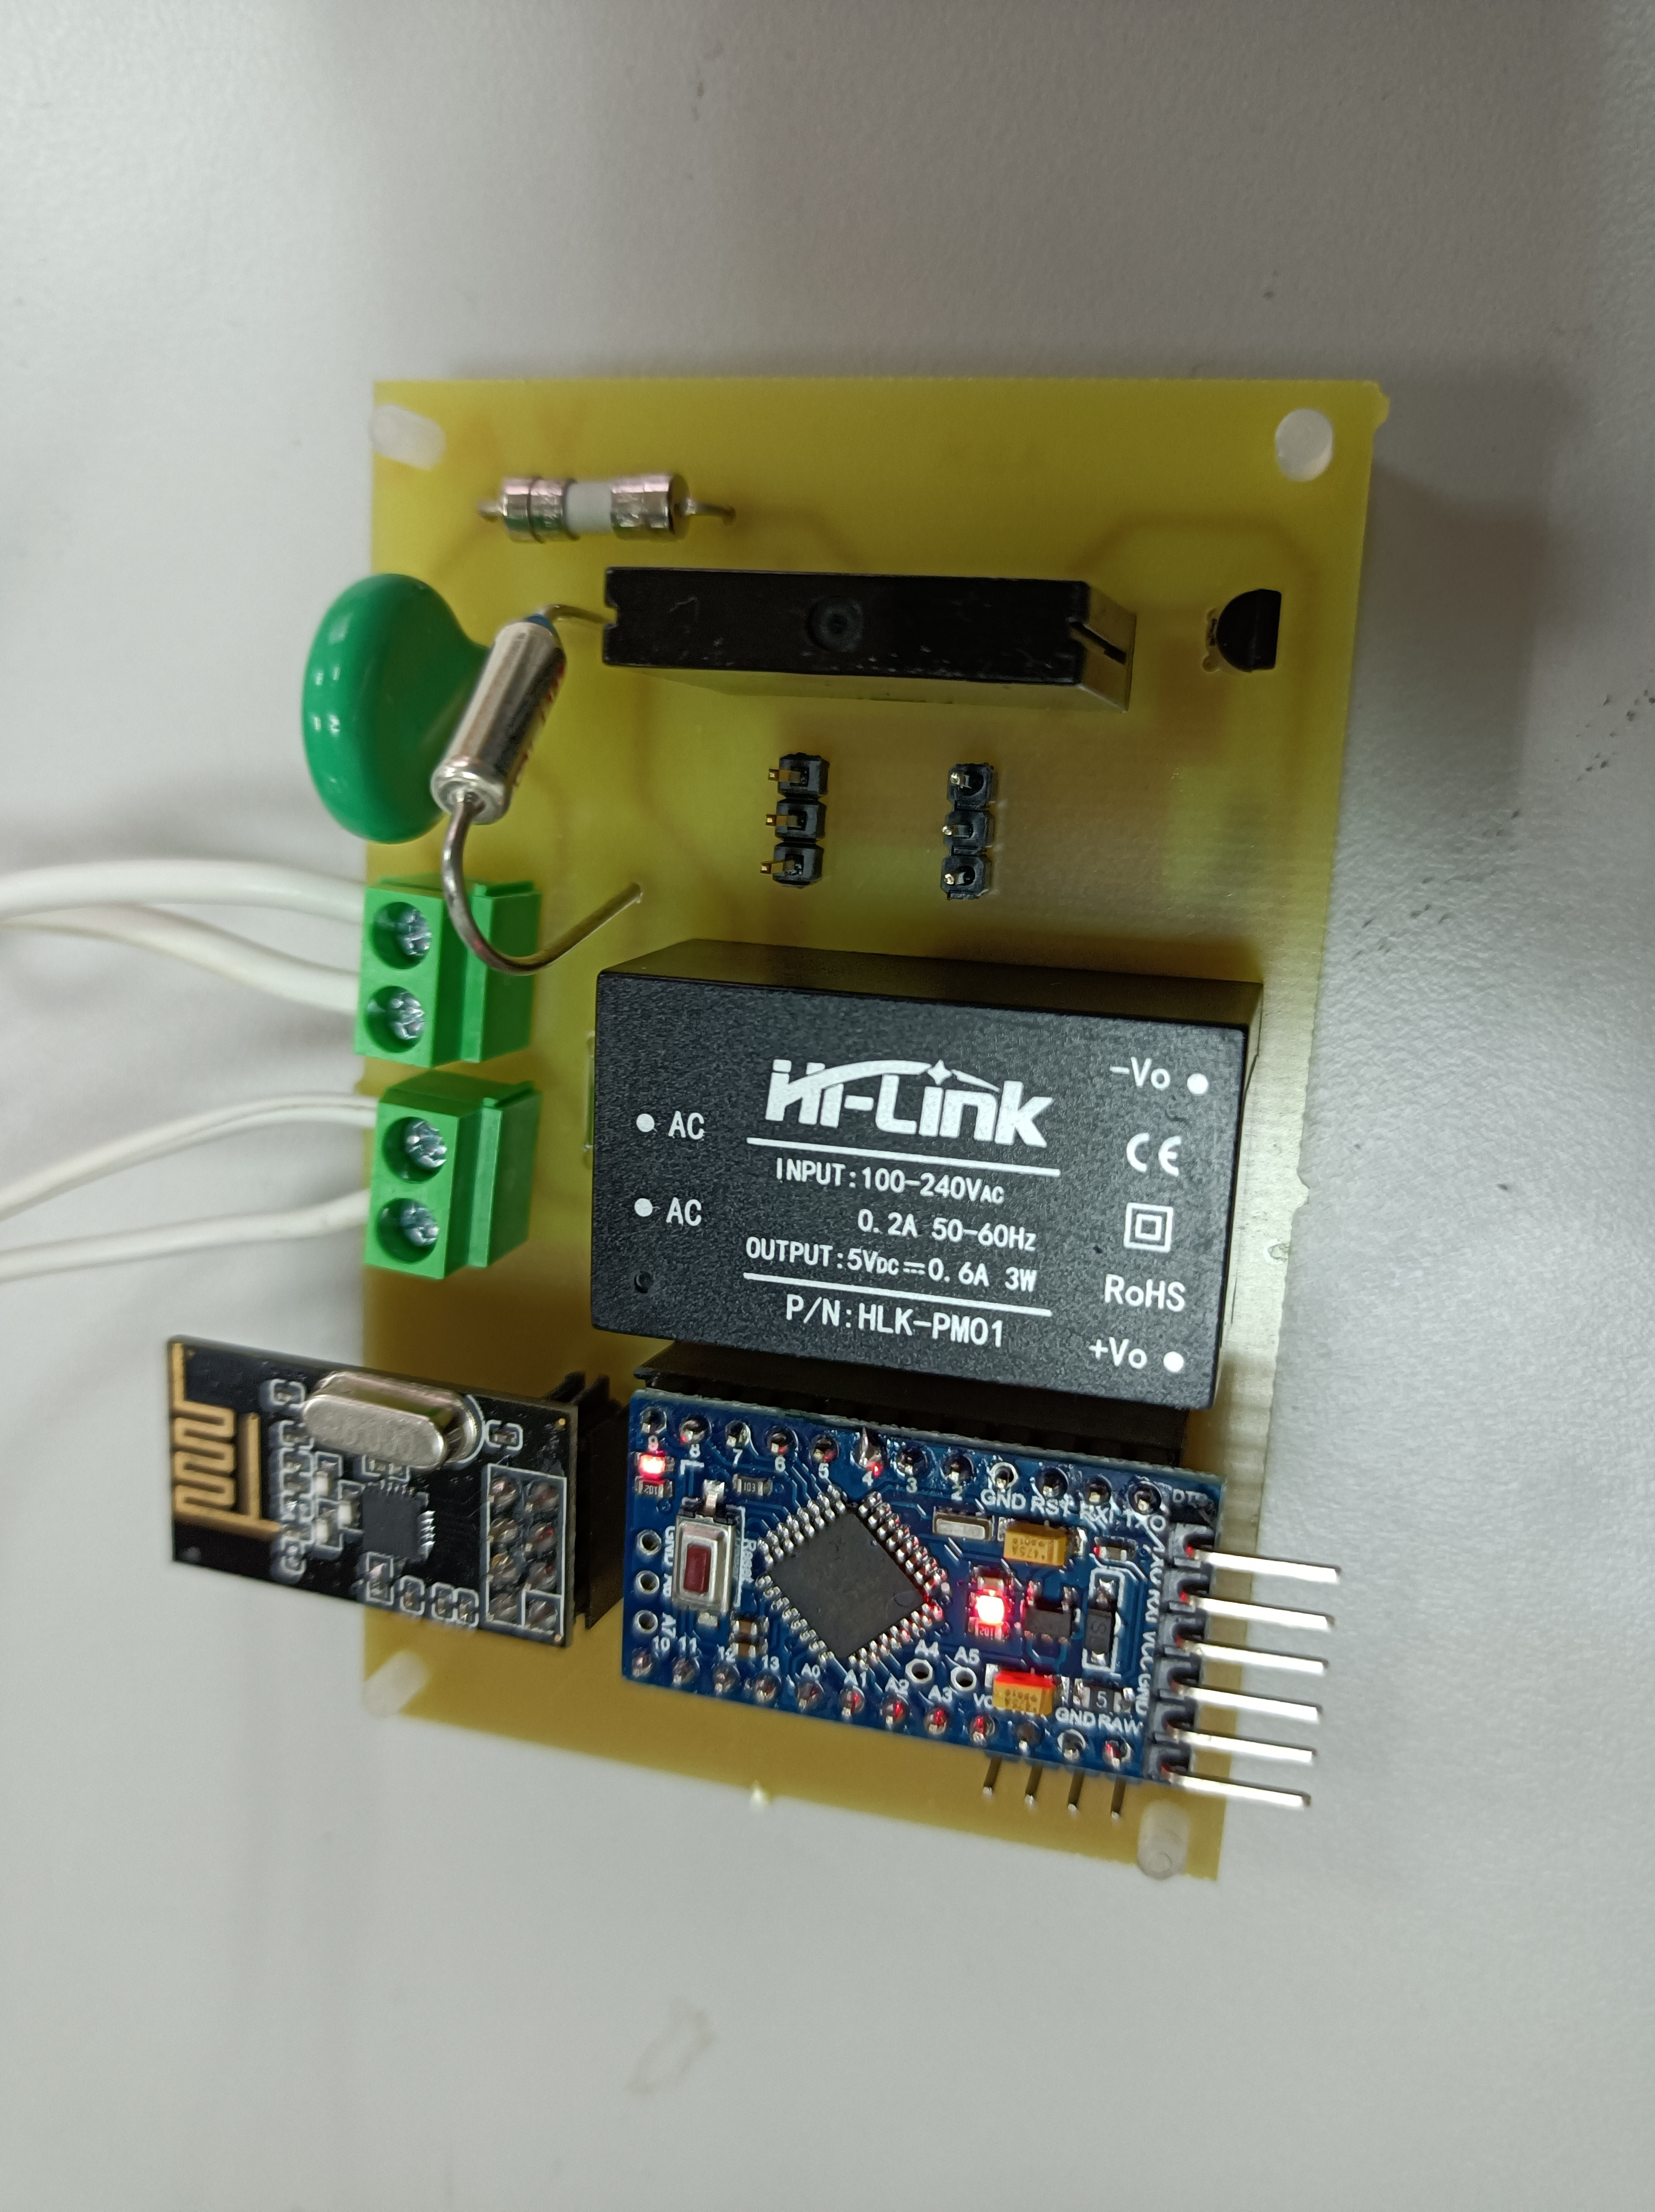
\includegraphics[width=\linewidth]{pcb-front.jpg}

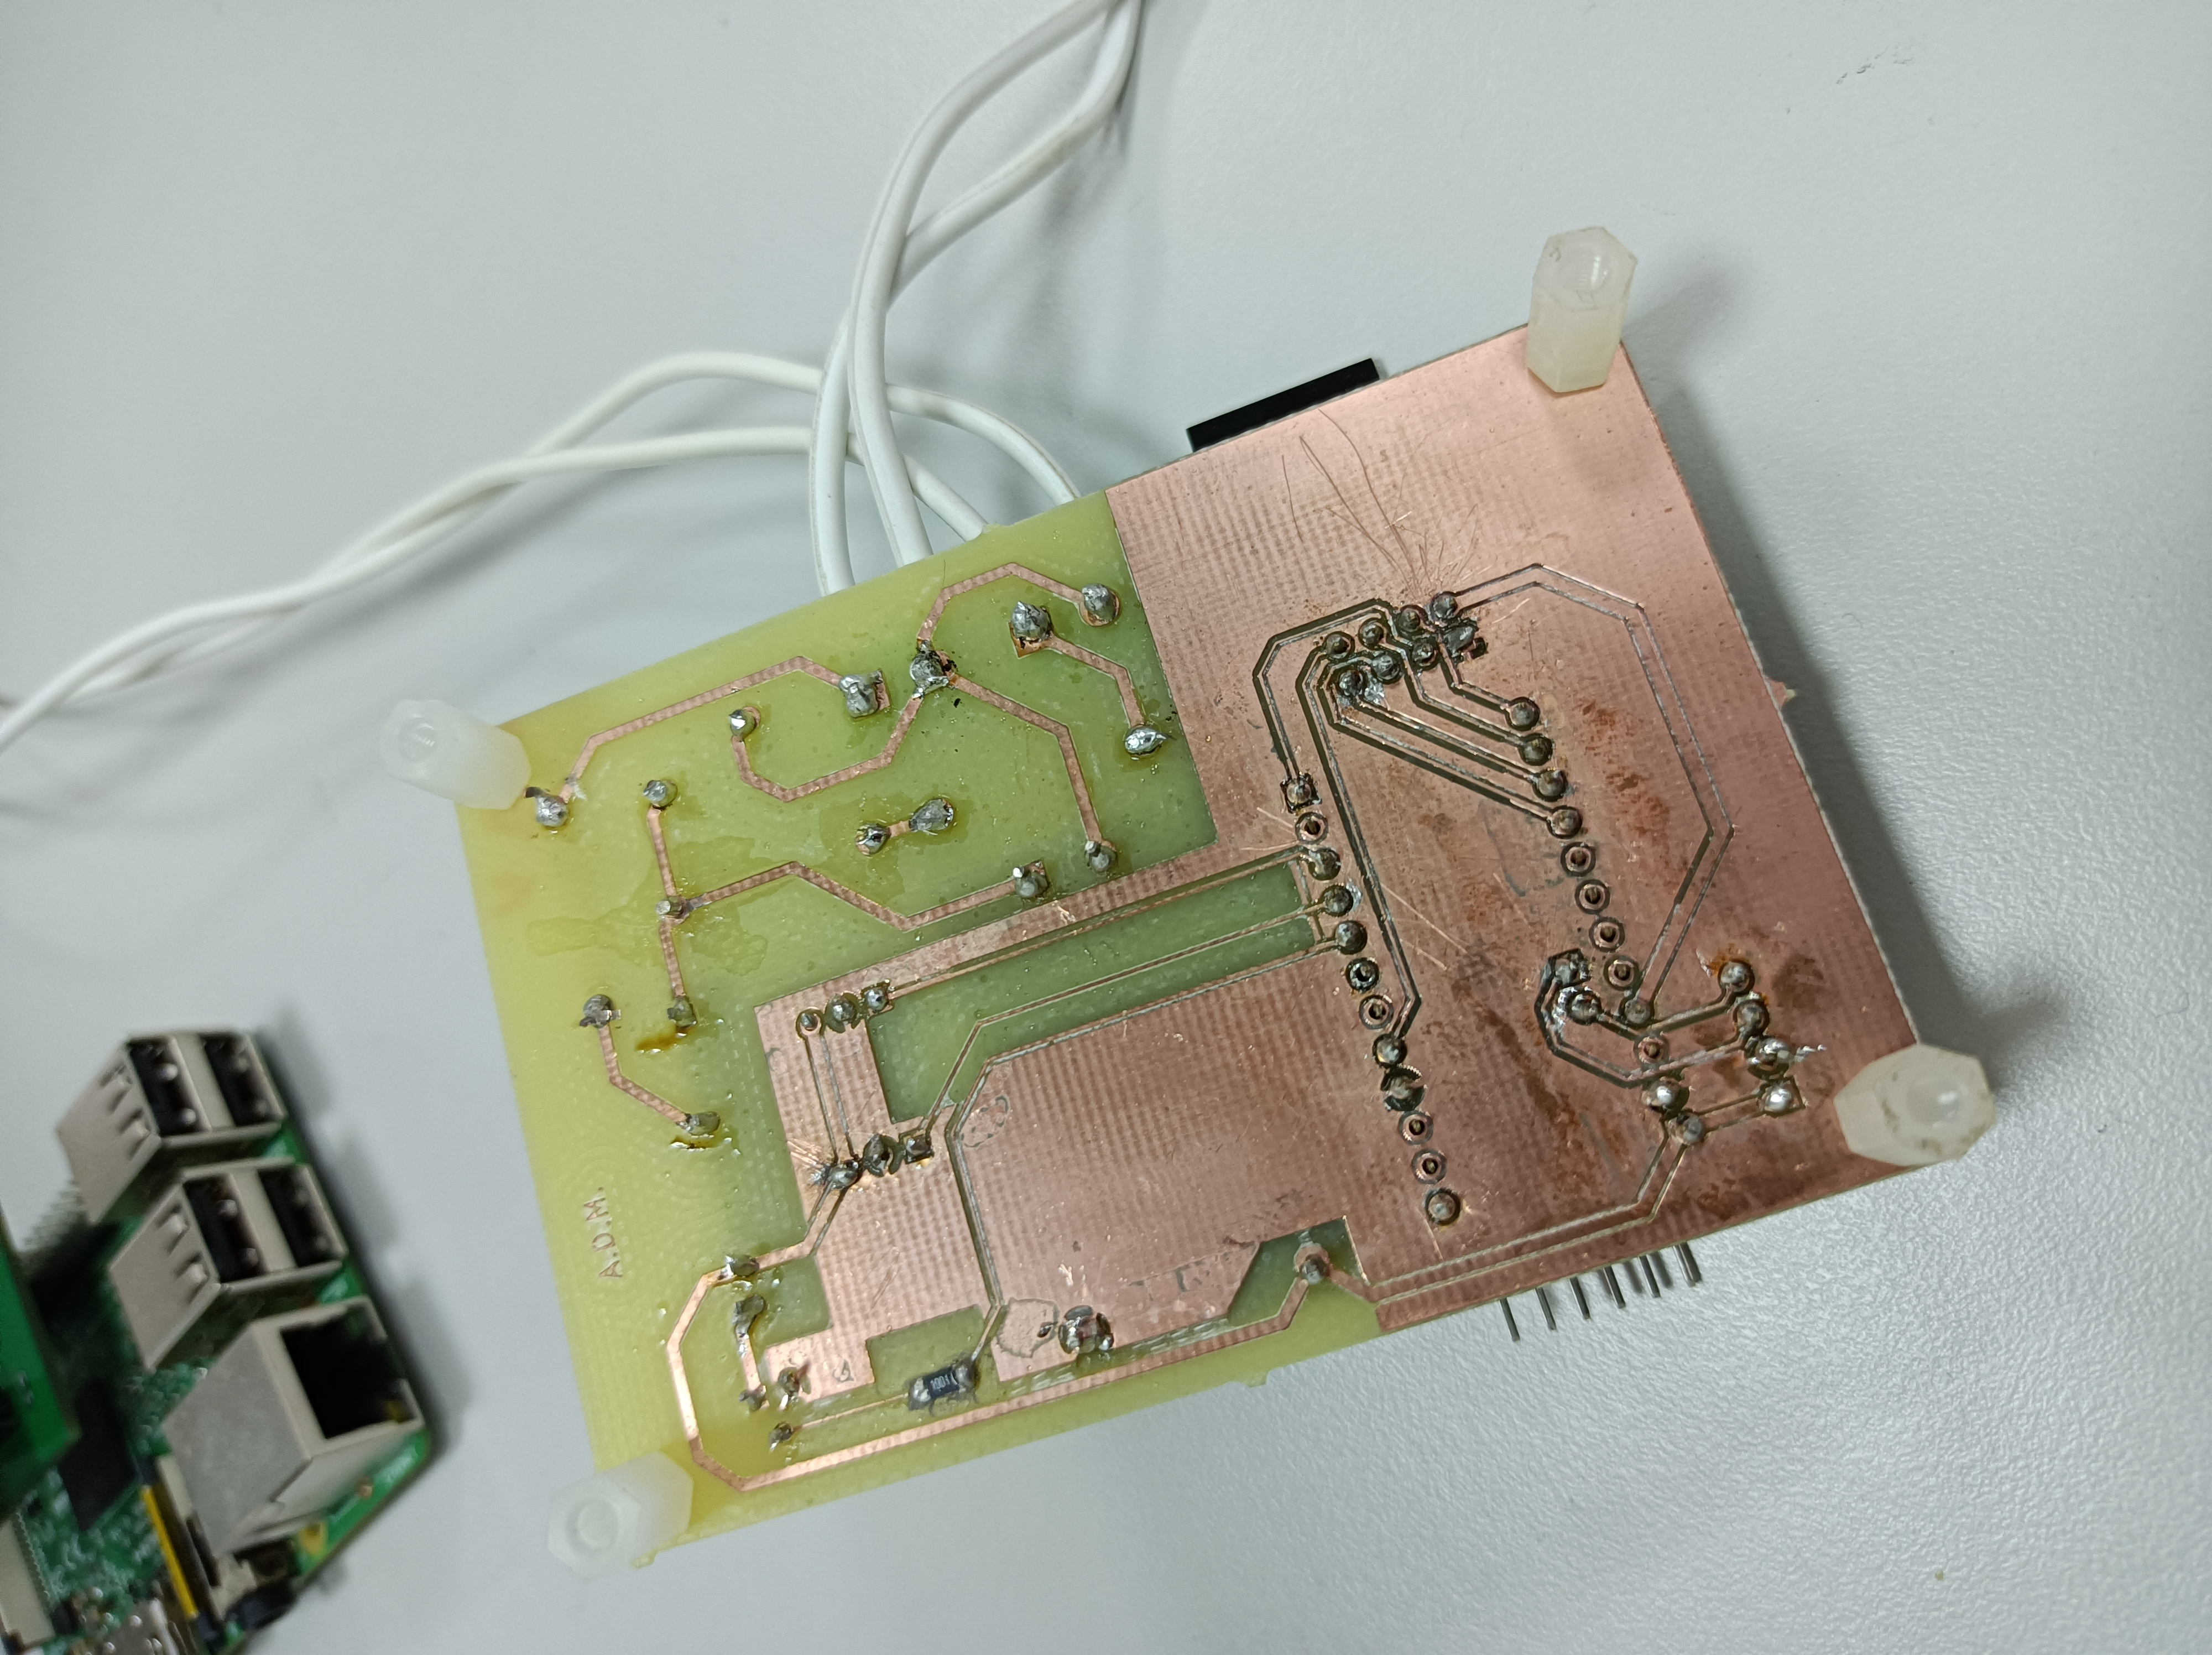
\includegraphics[width=\linewidth]{pcb-back.jpg}

Para ponerla a funcionar, hay que conectar uno de los terminales verdes a la
red doméstica y el otro a la luz o cualquier dispositivo preparado para
recibir 220 V de corriente alterna y no más de 2 A de intensidad. Con una luz
de tubo fluorescente encendida desde Domoticz queda así:

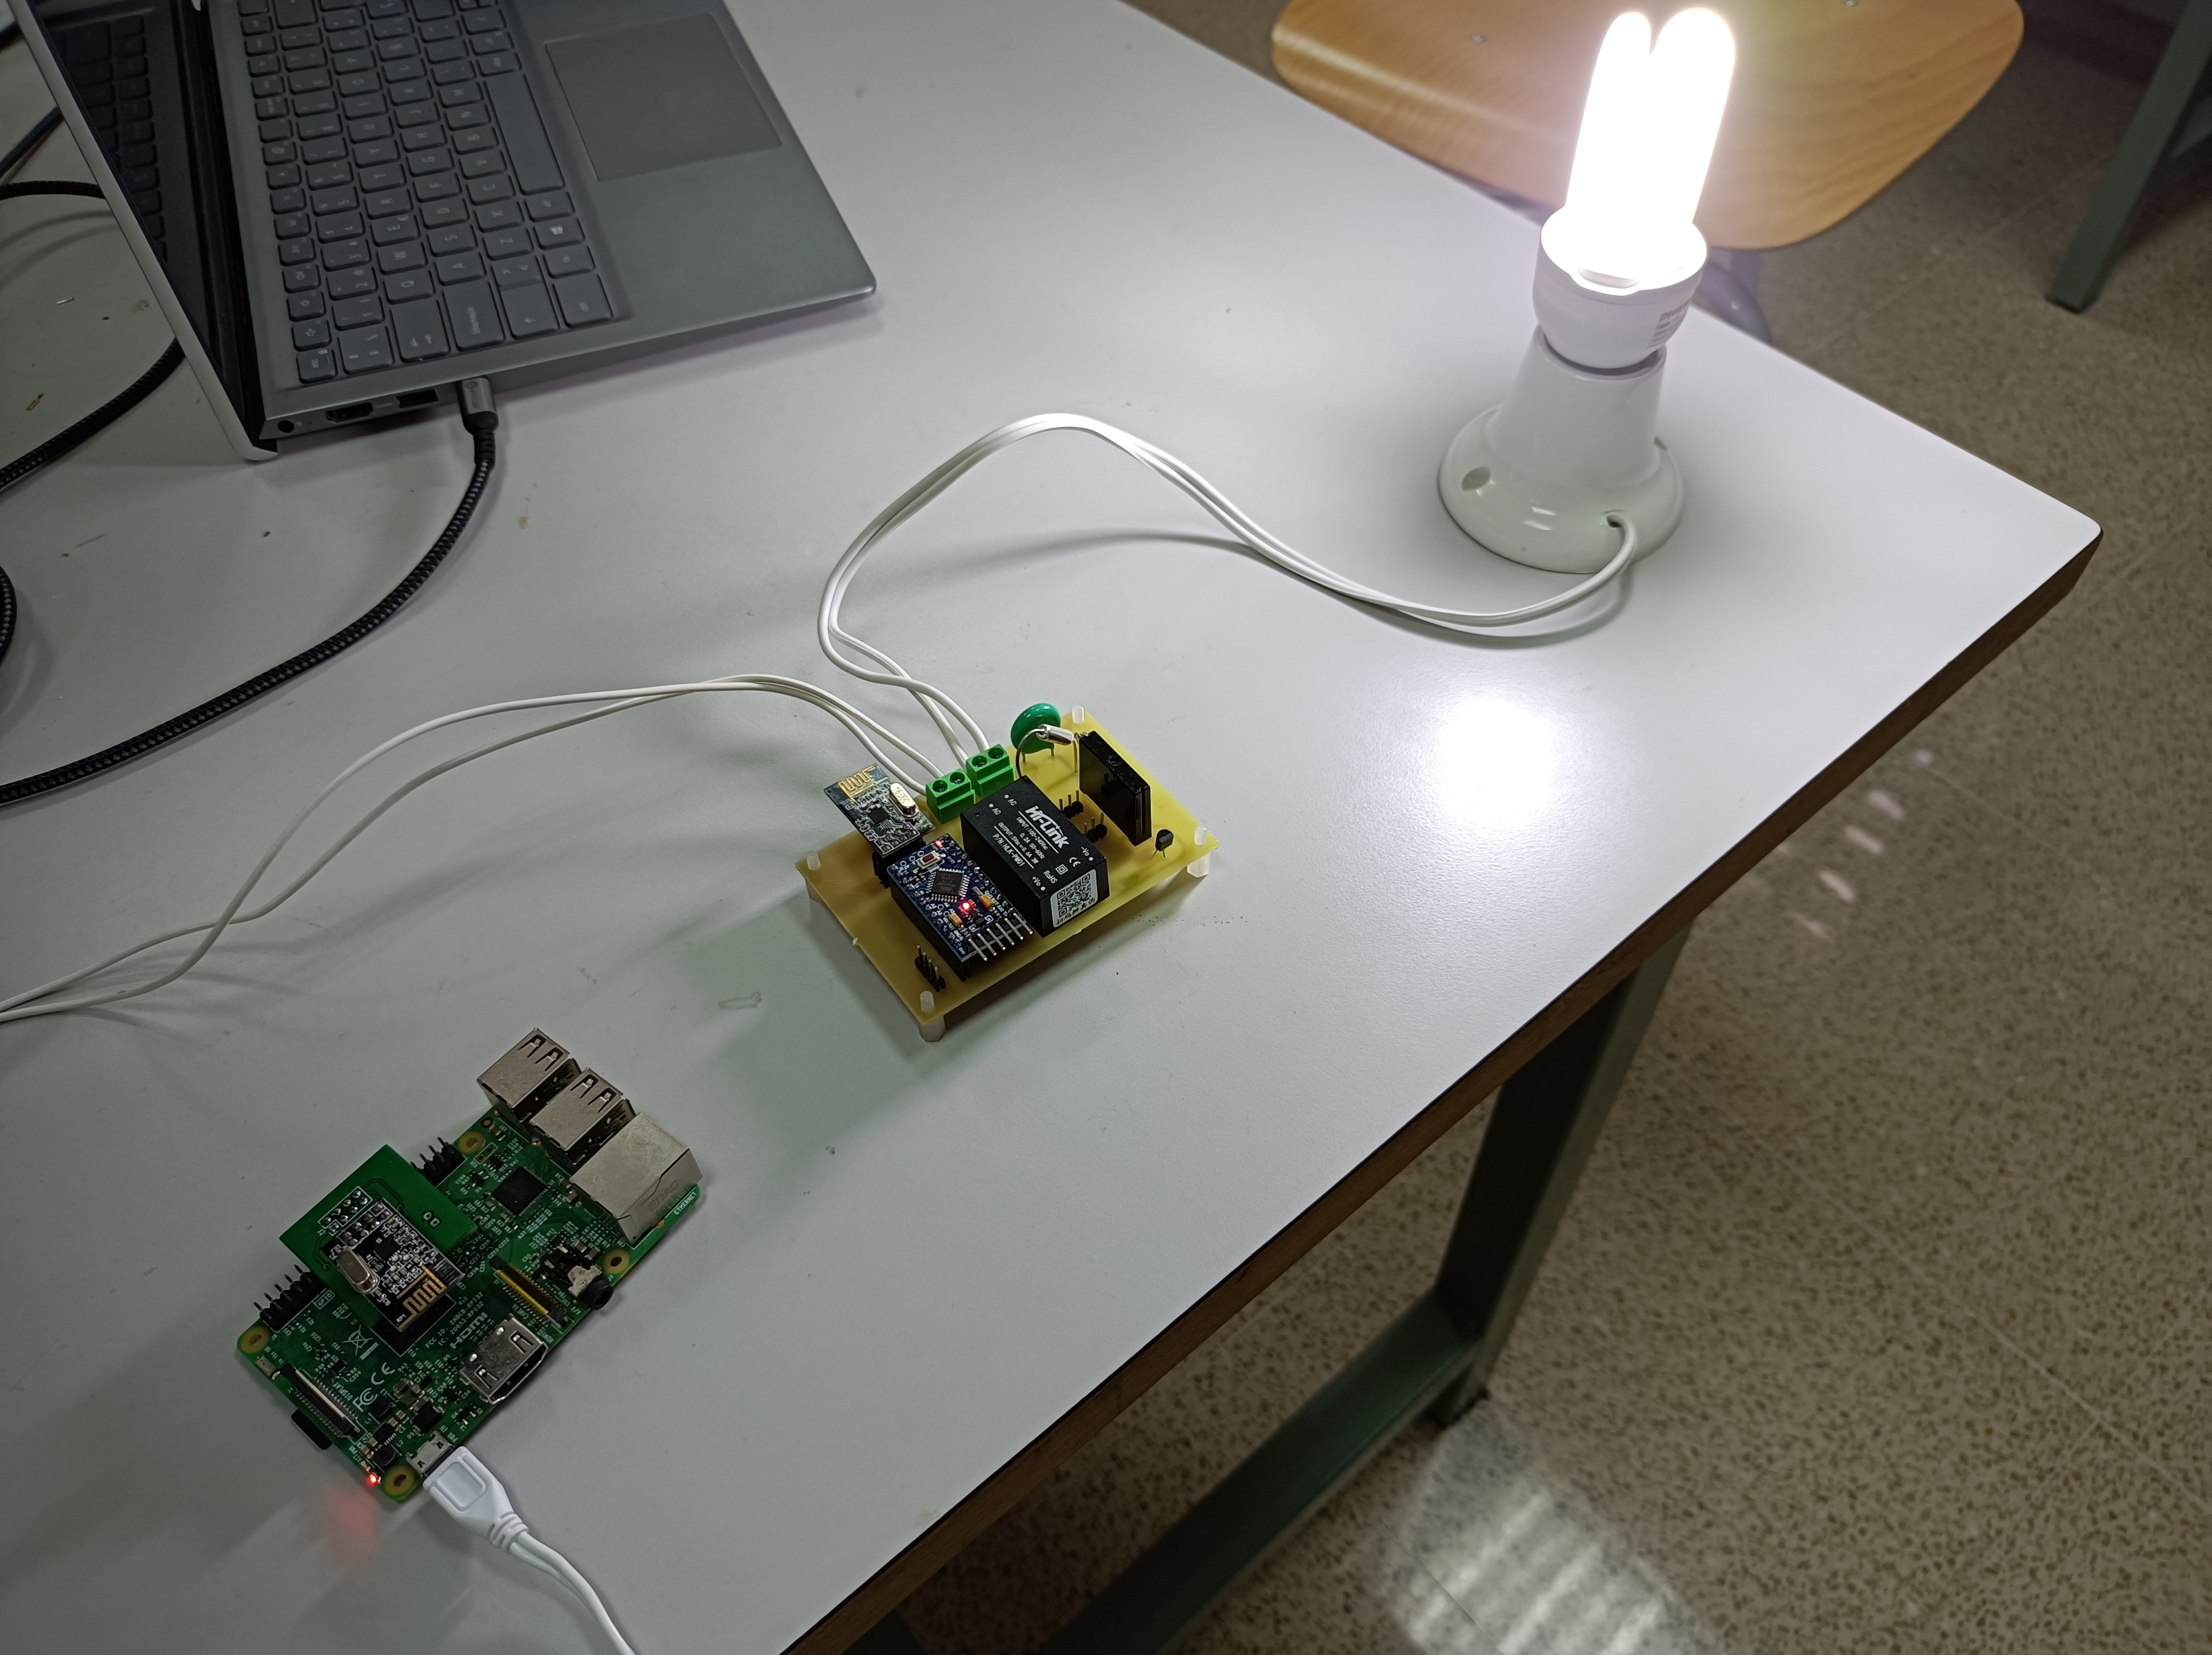
\includegraphics[width=\linewidth]{pcb-light-on.jpg}


\end{document}
